\documentclass[a4paper]{report}
\usepackage{setspace}

\pagestyle{plain}
\usepackage{amssymb,graphicx,color}
\usepackage{amsfonts}
\usepackage{booktabs}
\usepackage[section]{placeins}
\usepackage{latexsym}
\usepackage{amsmath}
\usepackage{tikz}
\usetikzlibrary{arrows.meta, positioning}
\usepackage[style=ieee, backend=biber]{biblatex}
\addbibresource{zotero.bib}
\usepackage{fancyvrb}
\usepackage{float}
\usepackage{multirow}
\usepackage{threeparttable}
\usepackage{pdfpages}
\usepackage{siunitx}
\usepackage[a4paper, margin = 3cm, bottom = 2.5cm]{geometry}
\usepackage{hyperref}

\newtheorem{theorem}{THEOREM}
\newtheorem{lemma}[theorem]{LEMMA}
\newtheorem{corollary}[theorem]{COROLLARY}
\newtheorem{proposition}[theorem]{PROPOSITION}
\newtheorem{remark}[theorem]{REMARK}
\newtheorem{definition}[theorem]{DEFINITION}
\newtheorem{fact}[theorem]{FACT}

\newtheorem{problem}[theorem]{PROBLEM}
\newtheorem{exercise}[theorem]{EXERCISE}
\def \set#1{\{#1\} }

\newenvironment{proof}{%
  PROOF: \begin{quotation}%
}{%
  $\Box$ \end{quotation}%
}

\newcommand{\nats}{\mbox{\( \mathbb N \)}}
\newcommand{\rat}{\mbox{\(\mathbb Q\)}}
\newcommand{\rats}{\mbox{\(\mathbb Q\)}}
\newcommand{\reals}{\mbox{\(\mathbb R\)}}
\newcommand{\ints}{\mbox{\(\mathbb Z\)}}

%%%%%%%%%%%%%%%%%%%%%%%%%%
\renewcommand{\thefootnote}{}


\title{{\vspace{-14em}}%
{{\Huge Spread Prediction for Portfolio Optimisation }}\\
{\large Evaluating whether spread prediction between cointegrated asset pairs produces more reliable return estimates than historical means for Markowitz optimisation }\\
}
\date{Submission date: 24th April 2026}
\author{Declan Loo\thanks{
{\bf Disclaimer:}
This report is submitted as part requirement for the BSc Degree in Computer Science at UCL. It is
substantially the result of my own work except where explicitly indicated in the text. The report may be freely copied and distributed provided the source is explicitly acknowledged.
}%
\\ \\
BSc Computer Science\\ \\
Supervisor's name: Dr. Tomaso Aste}

\begin{document}

\onehalfspacing
\maketitle
\begin{abstract}
Summarise your report concisely.
\end{abstract}

\tableofcontents
\setcounter{page}{1}


\chapter{Introduction}

This project uses only publicly available equity price data and does not involve human subjects, personal data, or data collection. No ethical approval was required for the project.

\section{Motivation}
Markowitz mean-variance optimisation \cite{markowitz1959} provides a rigorous framework for constructing efficient portfolios, yet its practical performance is highly sensitive to the accuracy of expected return estimates. Historical mean returns are extremely noisy estimators of future returns, with standard errors that often exceed the estimates themselves \cite{ledoit2004}, causing optimisers to produce unstable, concentrated allocations that perform poorly out-of-sample.
Cointegration-based pairs trading strategies exploit long-run equilibrium relationships between asset prices to generate mean-reverting spread signals \cite{gatev2006}. While extensive literature exists on pairs trading as a standalone strategy, few studies integrate spread-based predictions directly into the MPT framework as a systematic approach to return estimation.
This project addresses this gap by investigating whether the mean-reverting dynamics of cointegrated spreads, modelled via the Ornstein-Uhlenbeck process, can provide more reliable return signals for Markowitz optimisation than traditional historical means, thereby improving out-of-sample portfolio performance.

\section{Research Question}
Can spread prediction between cointegrated asset pairs provide more reliable return
estimates for Modern Portfolio Theory optimisation than traditional historical mean approaches?

\section{Research Hypothesis}
Spread-based return estimation derived from cointegrated asset pairs produces superior
portfolio allocations compared to historical mean-variance optimisation, measured by
risk-adjusted returns and portfolio stability, in terms of Sharpe ratio, volatility reduction
and maximum drawdown.

\section{Aims and Objectives}

The project has the following objectives:

\begin{itemize}
\item Develop a spread-based return estimation approach using cointegration analysis of asset
pairs that provides more stable signals than historical mean returns.
\item Build an integrated portfolio optimisation system using Markowitz framework and
validate through comprehensive back testing against traditional mean-variance
approaches using Sharpe ratio, volatility reduction, and drawdown metrics.
\item Create an interactive interface to demonstrate real-world applicability for portfolio
managers.
\end{itemize}

\section{Report Overview}

This report is structured as follows. Chapter~\ref{chap:background} provides the theoretical 
foundations underlying the project, covering Modern Portfolio Theory, the return estimation 
problem, cointegration theory, and the Ornstein-Uhlenbeck process. Chapter~\ref{chap:methodology} 
presents the methodology, detailing the cointegration screening procedure, spread modelling, 
OU-implied return estimation, and the minimum-variance portfolio optimisation framework. 
Chapter~\ref{chap:implementation} describes the implementation of the four-notebook pipeline, 
portfolio optimisation module, backtesting engine, and dashboard interface. 
Chapter~\ref{chap:results} presents the empirical results across cointegration screening, spread 
characterisation, out-of-sample validation, return estimation, and portfolio backtesting. 
Chapter~\ref{chap:discussion} interprets these results, addressing the central research question 
and examining the role of spread universe structure in driving performance. 
Chapter~\ref{chap:conclusions} summarises the achievements of the project, provides a critical 
evaluation, and outlines directions for future work.

\chapter{Background and Literature Review}
\label{chap:background}
This chapter reviews foundational theories underpinning the pairs trading strategy. Key concepts include Markowitz portfolio optimisation \cite{markowitz1959}, the return estimation problem, statistical arbitrage via pairs trading \cite{vidyamurthy2004}, cointegration (Engle-Granger) \cite{englegranger1987}, and the Ornstein--Uhlenbeck process for spread dynamics \cite{elliott2005}. These establish the theoretical framework for the methodology in Chapters ~\ref{chap:methodology} --~\ref{chap:results}.

\section{Mean-Variance Portfolio Optimisation}

Markowitz introduced Modern Portfolio Theory (MPT) in his seminal work \textit{Portfolio Selection: Efficient Diversification of Investments} \cite{markowitz1959}, establishing a quantitative framework for constructing optimal portfolios. MPT remains one of the most influential contributions to portfolio theory and optimisation, providing the theoretical foundation upon which much of modern finance is built. The theory characterises portfolio performance using two statistical measures: the mean as a proxy for expected return, and the standard deviation as a measure of risk. Within this framework, Markowitz defines a portfolio as \textbf{inefficient} if it is possible to achieve a higher expected return without increasing risk, or to reduce risk without sacrificing expected return. This gives rise to the \textit{Efficient Frontier}, the set of portfolios that offer the maximum expected return for a given level of risk, where any portfolio lying below the curve is considered suboptimal. The selection of an optimal portfolio along the frontier is determined by the investor's individual risk-return preference, reflecting the principle that higher expected returns are generally associated with greater risk. Central to MPT is also the principle of diversification: by combining assets whose returns are not perfectly correlated, investors can reduce overall portfolio risk without proportionally reducing expected return, since assets that do not move in perfect unison partially offset each other's fluctuations. This shifted the focus of portfolio construction from selecting individually attractive assets to engineering a portfolio whose constituent asset interactions collectively minimise risk — a conceptual shift that underpins virtually all modern asset allocation practice. 

However, MPT is not without limitations. Markowitz himself identified a fundamental shortcoming: the use of variance as the measure of risk was a pragmatic choice rather than a theoretically superior one. In his 1959 book, he explicitly argued that analyses based on semi-variance tend to produce \textit{``better portfolios''} than those based on variance \cite[p.~194]{markowitz1959}, since semi-variance captures only downside deviations --- the losses that investors genuinely seek to avoid --- whereas variance penalises upside and downside movements equally. Nevertheless, variance was retained on the grounds that it held an  advantage over semi-variance \textit{``with respect to cost, convenience, and familiarity''} \cite[p.~193]{markowitz1959}, particularly given the computational constraints of the era. A further, and arguably more practical, limitation of MPT is the instability of return estimation \cite{fabozzi2002}. Fabozzi, Gupta, and Markowitz demonstrate empirically that historical return estimates are highly sensitive to the time period selected: for instance, the MSCI Emerging Markets index returned 16.3\% annually over 1991--1995, yet only 0.1\% over 1996--2000 \cite[p.~9]{fabozzi2002}. The authors conclude that \textit{``there is no right answer because we are dealing with the world of uncertainty''} \cite[p.~9]{fabozzi2002}. Notwithstanding these limitations, they affirm that MPT \textit{``will occupy a permanent place in the theory and practice of finance''} \cite[p.~22]{fabozzi2002}. 

\section{The Return Estimation Problem}
\label{sec:return-estimation}

Historical mean returns are extremely noisy estimators of future returns, with standard errors that often exceed the estimates themselves \cite{ledoit2004}. As Merton (1980) demonstrates, even assuming a constant expected return, it would take a very long history of returns to obtain an accurate estimate due to the high volatility-to-sample-size ratio \cite{merton1980}. 

Brealey (1969) provides a foundational decomposition of stock price movements into four influences: (1) market-wide, (2) industry-specific, (3) subgroup, and (4) firm-specific factors. This suggests that stocks within the same industry share both market and industry systematic influences, making sector-paired stocks natural candidates for cointegration analysis \cite{brealey1969}. 

\section{Pairs Trading and Statistical Arbitrage}



\section{Cointegration Theory}

Engle and Granger introduced the concept of Cointegration where pairs that follow I(1) are deemed stationary if they pass the hypothesis tests deemed as the Engle-Granger test \cite{englegranger1987}. A study by 

\section{The Ornstein-Uhlenbeck Process}

Elliott in his Pairs Trading journal modelled the spread via the Ornstein-Uhlenbeck process \cite{elliott2005}

\section{Spread-Based Return Estimation}

\section{Summary}

\chapter{Methodology}
\label{chap:methodology}

This chapter details the methodology employed by this project. Section~\ref{sec:data_universe} describes the asset universe and data sourcing. Section~\ref{sec:coint_screening} presents the cointegration screening procedure used to identify suitable pairs. Sections~\ref{sec:spread_modelling} and~\ref{sec:return_estimation} develop the spread modelling and return estimation frameworks, respectively. Section~\ref{sec:portfolio_opt} formulates the portfolio optimisation problem, and Section~\ref{sec:backtesting} describes the backtesting framework used to evaluate performance.

\section{Data and Universe}
\label{sec:data_universe}

The project uses a \textbf{26-asset universe} of US equities (see Table ~\ref{tab:universe}). Stocks were selected on the basis of market capitalisation and sector-comembership, as economic similarity provides a prior expectation of long-run co-movement --- a necessary condition for cointegration. 

\begin{table}[htbp]
\centering
\caption{Investment Universe: 26 US Equities by Sector and Market Cap (29 Dec 2023)}
\label{tab:universe}
\footnotesize
\begin{tabular}{lllr}
\toprule
\textbf{Sector} & \textbf{Ticker} & \textbf{Name} & \textbf{Mkt Cap (\$B)} \\
\midrule
\multirow{4}{*}{Semiconductors}
  & NVDA.O  & Nvidia        & 1,223 \\
  & AMD.O   & AMD           & 238   \\
  & TSM.N   & TSMC          & 501   \\
  & INTC.O  & Intel         & 212   \\
\midrule
\multirow{4}{*}{Consumer Staples}
  & KO.N    & Coca-Cola     & 255   \\
  & PEP.O   & PepsiCo       & 234   \\
  & COST.O  & Costco        & 293   \\
  & TGT.N   & Target        & 66    \\
\midrule
\multirow{4}{*}{Financials}
  & JPM.N   & JPMorgan Chase& 492   \\
  & BAC.N   & Bank of America& 266  \\
  & GS.N    & Goldman Sachs & 126   \\
  & MS.N    & Morgan Stanley& 153   \\
\midrule
\multirow{4}{*}{Energy}
  & XOM.N   & ExxonMobil    & 400   \\
  & CVX.N   & Chevron       & 281   \\
  & SLB.N   & Schlumberger  & 74    \\
  & HAL.N   & Halliburton   & 32    \\
\midrule
\multirow{2}{*}{Airlines}
  & DAL.N   & Delta Air Lines & 26  \\
  & UAL.O   & United Airlines & 14  \\
\midrule
\multirow{4}{*}{E-Commerce/Cloud}
  & AMZN.O  & Amazon        & 1,570 \\
  & MSFT.O  & Microsoft     & 2,795 \\
  & META.O  & Meta          & 910   \\
  & GOOGL.O & Alphabet      & 1,755 \\
\midrule
\multirow{4}{*}{Healthcare}
  & JNJ.N   & Johnson \& Johnson & 377 \\
  & PFE.N   & Pfizer        & 163   \\
  & MRK.N   & Merck         & 276   \\
  & ABBV.N  & AbbVie        & 274   \\
\bottomrule
\end{tabular}
\end{table}

From these 26 stocks, 16 candidate pairs are pre-selected within sectors. Restricting pair formation to within-sector groupings reflects the economic rationale that stocks exposed to common demand drivers, regulatory environments, and supply chains tend to co-move \cite{brealey1969} and are therefore more likely to exhibit the long-run equilibrium relationship required for cointegration. (see Section~\ref{sec:return-estimation}). 

Daily adjusted close prices are sourced from LSEG Data Library \cite{lsegdata2025}. S\&P 500 benchmark returns are obtained via the \texttt{yfinance} \cite{yfinance2026} library. The full sample spans 1 January 2018 to 31 December 2025 and is partitioned into: 

\begin{itemize} 
\item \textbf{In-Sample (IS)}: 1 January 2018 -- 31 December 2023 (cointegration screening, calibration) 
\item \textbf{Out-of-Sample (OOS)}: 1 January 2024 -- 31 December 2025 (backtesting) 
\end{itemize} 

This IS/OOS split ensures that all model parameters are estimated without look-ahead bias. 

\section{Cointegration Screening}
\label{sec:coint_screening}

The cointegration screening pipeline identifies which of the 16 candidate pairs exhibit a statistically significant long-run equilibrium relationship, following the two-step Engle--Granger procedure \cite{englegranger1987}.

\subsection{Unit Root Testing}

A prerequisite for cointegration is that each of the individual price series is integrated of order one, denoted $I(1)$: non-stationary in levels, but stationary in first differences ($\Delta P_t = P_t - P_{t-1}$). For each stock, the Augmented Dickey-Fuller (ADF) test is applied to both the level series $P_t$ and its first order $\Delta P_t$. A series is classified $I(1)$ if 

\begin{enumerate} 
    \item ADF on levels \textbf{fails to reject} unit root ($p > 0.05$), \textbf{suggesting non-stationarity}, 
    \item ADF on $\Delta P_t$ \textbf{rejects} unit root ($p \leq 0.05$), indicating stationarity. 
\end{enumerate} 

The ADF regression is: 
\begin{equation}
\Delta P_t = \alpha + \gamma P_{t-1} + \sum_{j=1}^{p} \delta_j \Delta P_{t-j} + \varepsilon_t 
\end{equation}

where $\Delta P_t = P_t - P_{t-1}$ (first difference), $\alpha$ is the constant, $\gamma$ tests the unit root ($H_0: \gamma = 0$), $\delta_j$ are lag coefficients, and $\varepsilon_t \sim N(0,\sigma^2)$ is white noise. Lag order $p$ is selected via Akaike Information Criterion (AIC). Only pairs where both stocks are $I(1)$ proceed to cointegration testing. 

\subsection{Engle--Granger Procedure}

For each candidate pair $(Y_t, X_t)$ passing the $I(1)$ filter, the Engle--Granger two-step procedure \cite{englegranger1987} is applied:

\paragraph{Step 1: Cointegrating regression.} With $Y_t$ as dependent variable and $X_t$ as independent variable, estimate the static OLS regression over the in-sample period:
\begin{equation}
Y_t = \alpha + \beta X_t + \epsilon_t \label{eq:coint_regression}
\end{equation}
where $\beta$ is the hedge ratio and $\alpha$ the intercept.

\paragraph{Step 2: Residual stationarity test.} Apply the ADF test to OLS residuals $\hat{\epsilon}_t = Y_t - \hat{\alpha} - \hat{\beta} X_t$. Because residuals are estimated, standard ADF critical values are inappropriate; \textbf{MacKinnon critical values} \cite{mackinnon2010} are used instead, accounting for estimation uncertainty.

To avoid ordering effects, both $(Y|X)$ and $(X|Y)$ are tested; the ordering with the lowest residual ADF $p$-value is retained. A pair is deemed cointegrated if $p < 0.05$.

\section{Spread Modelling}
\label{sec:spread_modelling}

For each cointegrated pair, the spread is constructed and its mean-reverting dynamics are characterised.

\subsection{OLS Residual Spread}

The spread is defined as the residual from the cointegrating regression:
\begin{equation}
S_t = Y_t - \hat{\beta} X_t - \hat{\alpha}
\label{eq:spread}
\end{equation}
where $\hat{\beta}$ and $\hat{\alpha}$ are estimated from the in-sample OLS regression (Equation~\ref{eq:coint_regression}). Under the cointegration hypothesis, $S_t$ is a stationary, mean-reverting process fluctuating around zero.

\subsection{Half-Life and Hurst Exponent}

Two complementary diagnostics quantify the strength and speed of mean reversion.

\paragraph{Half-life of mean reversion.} Following pairs trading convention \cite{gatev2006}, model the spread as a discrete-time AR(1):
\begin{equation}
\Delta S_t = \lambda S_{t-1} + \varepsilon_t \label{eq:ar1}
\end{equation}
where $\lambda < 0$ implies mean reversion to $\mu = 0$. Half-life:
\begin{equation}
h = -\frac{\ln 2}{\ln(1 + \lambda)} \approx -\frac{\ln 2}{\lambda} \label{eq:halflife}
\end{equation}

Shorter half-lives indicate faster mean reversion and are preferable for trading. The approximation $\ln(1+\lambda) \approx \lambda$ is valid for $|\lambda| \ll 1$.

\paragraph{Hurst exponent.} The Hurst exponent $H$ is estimated via the variogram method. For a time series $\{S_t\}$, the variogram at lag $\tau$ is:
\begin{equation}
V(\tau) = \mathbb{E}\left[(S_{t+\tau} - S_t)^2\right]
\label{eq:variogram}
\end{equation}
For a fractional process, $V(\tau) \propto \tau^{2H}$, so $H$ is estimated by regressing $\log V(\tau)$ on $\log \tau$ and halving the slope. A Hurst exponent $H < 0.5$ indicates mean-reverting behaviour, $H = 0.5$ corresponds to a random walk, and $H > 0.5$ indicates trending behaviour. Pairs are retained only if $H < 0.5$, providing an independent confirmation of mean reversion beyond the ADF test.

\subsection{Rolling Z-Score}

To generate trading signals that adapt to time-varying spread dynamics, a rolling $z$-score is computed:
\begin{equation}
z_t = \frac{S_t - \bar{S}_t^{(w)}}{\sigma_t^{(w)}}
\label{eq:zscore}
\end{equation}
where $\bar{S}_t^{(w)}$ and $\sigma_t^{(w)}$ denote the rolling mean and standard deviation of the spread over a trailing window of $w = 60$ trading days. The rolling window allows the signal to adapt to structural shifts in spread dynamics while remaining responsive to short-term dislocations.

\section{Return Estimation}
\label{sec:return_estimation}

This section develops the two competing approaches to estimating expected returns for portfolio optimisation: the proposed OU-implied method and the traditional historical mean baseline.

\subsection{OU-Implied Expected Returns}

The core contribution of this project is to derive expected returns from the mean-reverting dynamics of cointegrated spreads. The Ornstein--Uhlenbeck (OU) process \cite{elliott2005} provides the continuous-time model for the spread:
\begin{equation}
dS_t = \kappa(\theta - S_t)\,dt + \sigma\,dW_t
\label{eq:ou_sde}
\end{equation}
where $\kappa > 0$ is the speed of mean reversion, $\theta$ is the long-run equilibrium level, and $\sigma$ is the diffusion coefficient. The parameter $\kappa$ is related to the discrete-time half-life (Equation~\ref{eq:halflife}) by:
\begin{equation}
\kappa = \frac{\ln 2}{h}
\label{eq:kappa}
\end{equation}

The expected change in the spread over a single period, conditional on the current spread level $S_t$, is:
\begin{equation}
\mathbb{E}[\Delta S_{t+1} \mid S_t] = (\theta - S_t)\left(1 - e^{-\kappa}\right)
\label{eq:ou_expected_return}
\end{equation}

This expression captures the key economic intuition: when the spread is below its equilibrium ($S_t < \theta$), the expected change is positive (reversion upward), and vice versa. The magnitude of the expected return is proportional to both the displacement from equilibrium and the speed of mean reversion.

The spread return for a pair $(Y, X)$ with hedge ratio $\beta$ is defined as:
\begin{equation}
r_t^{S} = \ln\!\left(\frac{Y_t}{Y_{t-1}}\right) - \beta \cdot \ln\!\left(\frac{X_t}{X_{t-1}}\right)
\label{eq:spread_return}
\end{equation}

The OU-implied expected spread return is then used as the expected return vector $\boldsymbol{\mu}$ in the portfolio optimisation framework (Section~\ref{sec:portfolio_opt}).

\subsection{Historical Mean Returns}

As a baseline, expected returns are estimated using the sample mean of realised spread returns over the in-sample period:
\begin{equation}
\hat{\mu}_i = \frac{1}{T}\sum_{t=1}^{T} r_{i,t}^{S}
\label{eq:hist_mean}
\end{equation}
This estimator is unbiased but has high variance---a well-documented limitation in portfolio optimisation \cite{merton1980}. Comparing portfolio performance under OU-implied versus historical mean return estimates provides a direct test of the research hypothesis.

\section{Portfolio Optimisation}
\label{sec:portfolio_opt}

Given a vector of expected spread returns $\boldsymbol{\mu} \in \mathbb{R}^n$ and a covariance matrix $\boldsymbol{\Sigma} \in \mathbb{R}^{n \times n}$ for $n$ spread strategies, the portfolio allocation problem is cast in the Markowitz mean-variance framework \cite{markowitz1959}.

\subsection{Minimum-Variance Formulation}

The minimum-variance portfolio solves:
\begin{equation}
\begin{aligned}
\min_{\mathbf{w}} \quad & \mathbf{w}^\top \boldsymbol{\Sigma} \mathbf{w} + \delta \|\mathbf{w}\|_2^2 \\
\text{subject to} \quad & \mathbf{1}^\top \mathbf{w} = 1, \\
& w_i \geq 0 \quad \forall\, i
\end{aligned}
\label{eq:min_var}
\end{equation}
where $\delta \geq 0$ is an optional $L_2$ regularisation parameter that penalises concentrated allocations and improves numerical stability when $\boldsymbol{\Sigma}$ is near-singular.

The maximum Sharpe ratio portfolio maximises:
\begin{equation}
\max_{\mathbf{w}} \quad \frac{\mathbf{w}^\top \boldsymbol{\mu} - r_f}{\sqrt{\mathbf{w}^\top \boldsymbol{\Sigma} \mathbf{w}}}
\label{eq:max_sharpe}
\end{equation}
subject to the same long-only and full-investment constraints. Here $r_f = 0.02$ denotes the annualised risk-free rate.

The covariance matrix $\boldsymbol{\Sigma}$ is estimated using the Ledoit--Wolf shrinkage estimator, which linearly combines the sample covariance with a structured target (the identity matrix scaled by the average variance). This addresses the well-known instability of sample covariance matrices in moderate-dimensional settings by shrinking extreme eigenvalues towards a more stable structure.

Expected returns are annualised from daily log returns via the transformation $\mu_{\text{ann}} = \exp(252 \cdot \mu_{\text{daily}}) - 1$, and volatilities are annualised as $\sigma_{\text{ann}} = \sigma_{\text{daily}} \cdot \sqrt{252}$.

\subsection{Spread Space vs Asset Space}

A distinctive feature of this methodology is that optimisation is performed in \emph{spread space} rather than directly over individual assets. Each dimension of the portfolio vector $\mathbf{w}$ corresponds to a spread strategy (a cointegrated pair), not an individual stock. This has several advantages:
\begin{itemize}
    \item \textbf{Dimensionality reduction}: the number of spreads (up to 16) is smaller than the number of assets (26), yielding a lower-dimensional and better-conditioned optimisation problem.
    \item \textbf{Built-in hedging}: each spread is by construction a hedged position (long one leg, short the other by $\beta$ units), so the portfolio inherits partial market-neutrality.
    \item \textbf{Signal coherence}: the OU-implied return estimates are naturally defined at the spread level, avoiding the need to decompose spread-level predictions back into asset-level expected returns.
\end{itemize}

The weight $w_i$ allocated to spread $i$ determines the fraction of capital deployed to that pair strategy. The resulting portfolio return on day $t$ is $r_t^P = \sum_i w_i \cdot r_{i,t}^{S}$.

\section{Backtesting Framework}
\label{sec:backtesting}

The backtesting engine simulates a $z$-score-based mean-reversion strategy for each pair, then evaluates the optimised portfolio of pair strategies against benchmarks.

\subsection{In-Sample / Out-of-Sample Split}

The temporal split is strict: the in-sample period (1 January 2018 -- 31 December 2023) is used for all estimation---cointegrating regressions, hedge ratios, OU parameters, spread statistics, and portfolio weights. The out-of-sample period (1 January 2024 -- 31 December 2025) is used exclusively for performance evaluation. No re-estimation or recalibration is performed during the OOS period, ensuring a clean test of whether in-sample model parameters generalise.

\paragraph{Pair-level signal generation.} For each pair, a position signal is generated using a $z$-score state machine with three thresholds:
\begin{itemize}
    \item \textbf{Entry} ($|z_t| \geq z_{\text{entry}} = 2.0$): open a position when the spread is sufficiently dislocated. If $z_t \leq -z_{\text{entry}}$, go long the spread (expecting reversion upward); if $z_t \geq z_{\text{entry}}$, go short the spread.
    \item \textbf{Exit} ($|z_t| \leq z_{\text{exit}} = 0.0$): close the position when the spread has reverted to its rolling mean.
    \item \textbf{Stop-loss} ($|z_t| \geq z_{\text{stop}} = 4.0$): force-close the position if the spread diverges further, limiting downside risk.
\end{itemize}

\paragraph{Position sizing and transaction costs.} The full initial capital ($C_0 = \$100{,}000$) is deployed into each active spread position. One spread unit costs $Y_t + |\beta| \cdot X_t$ in notional terms, and the number of units is $n_t = C_0 / (Y_t + |\beta| X_t)$. Transaction costs of $c = 10$ basis points are incurred proportionally on each position change. The daily strategy return is:
\begin{equation}
r_t = \frac{\text{pos}_{t-1} \cdot n_{t-1} \cdot (\Delta Y_t - \beta \cdot \Delta X_t) - \text{TC}_t}{C_0}
\label{eq:backtest_return}
\end{equation}
where $\text{TC}_t = |\Delta \text{pos}_t| \cdot C_0 \cdot (c / 10{,}000)$.

\subsection{Evaluation Metrics}

Portfolio performance is assessed using the following metrics:

\paragraph{Annualised Sharpe ratio.} The ex-post Sharpe ratio is computed as:
\begin{equation}
\text{SR} = \frac{\bar{r} - r_f / 252}{\sigma_r} \cdot \sqrt{252}
\label{eq:sharpe}
\end{equation}
where $\bar{r}$ is the mean daily return, $r_f = 0.02$ is the annualised risk-free rate, and $\sigma_r$ is the standard deviation of daily returns.

\paragraph{Maximum drawdown.} The maximum peak-to-trough decline in cumulative returns:
\begin{equation}
\text{MDD} = \max_{t} \left(\frac{\max_{\tau \leq t} V_\tau - V_t}{\max_{\tau \leq t} V_\tau}\right)
\label{eq:mdd}
\end{equation}
where $V_t$ is the cumulative portfolio value at time $t$.

\paragraph{Volatility reduction.} The percentage reduction in annualised volatility relative to an equal-weight buy-and-hold benchmark of the constituent stocks:
\begin{equation}
\text{VR} = 1 - \frac{\sigma_{\text{strategy}}}{\sigma_{\text{benchmark}}}
\label{eq:vol_reduction}
\end{equation}

\paragraph{Additional metrics.} Win rate (fraction of active trading days with positive returns), profit factor (ratio of gross profits to gross losses), number of round-trip trades, and total return are also reported.

\paragraph{Benchmarks.} Three benchmarks are used for comparison: (i)~an equal-weight buy-and-hold portfolio of all universe constituents, (ii)~individual buy-and-hold of each pair leg, and (iii)~the S\&P~500 index as a broad market proxy.

\subsection{Statistical Robustness Tests}

Three additional tests are applied to the OOS results to assess statistical robustness:

\paragraph{Bootstrap confidence intervals.} Given the short OOS window ($T \approx 501$ trading days), point Sharpe ratio estimates carry high sampling variance. Bootstrap confidence intervals are constructed by resampling daily returns with replacement 10{,}000 times, providing empirical 95\% CIs for each strategy's Sharpe ratio.

\paragraph{Paired significance test.} A paired $t$-test and non-parametric Wilcoxon signed-rank test are applied to the daily return difference between OU Max-Sharpe and Historical Max-Sharpe. This directly tests whether the observed Sharpe advantage of the OU-Implied approach is statistically significant or within normal sampling variation.

\paragraph{Sensitivity analysis.} The per-pair backtest is re-run across a grid of entry $z$-scores $\{1.5, 2.0, 2.5, 3.0\}$ and transaction costs $\{0, 5, 10, 20, 30\}$ bps, assessing whether conclusions are robust to parameter choice. A leave-one-pair-out (LOPO) test additionally re-optimises the portfolio after removing each pair, verifying that the full-portfolio result is not dominated by a single spread.

\section{Summary}

This chapter has presented the complete methodology for the project. The pipeline proceeds from data sourcing and cointegration screening, through spread modelling and OU-implied return estimation, to Markowitz portfolio optimisation and rigorous out-of-sample backtesting. The key methodological contribution is the use of OU-implied expected returns derived from cointegrated spreads as inputs to the mean-variance optimiser, compared against a traditional historical mean baseline. Chapter~\ref{chap:implementation} describes how this methodology is implemented in software.

\chapter{Implementation}
\label{chap:implementation}

This chapter describes the software implementation of the methodology presented in Chapter~\ref{chap:methodology}. The system is implemented in Python and organised into a modular pipeline of reusable library code, analysis notebooks, a backtesting engine, and an interactive dashboard. All source code is available at the project repository.

\section{Pipeline Overview}
\label{sec:pipeline_overview}

The project follows a four-stage notebook pipeline, each building on the outputs of the previous stage, supported by three library packages (\texttt{src/modelling}, \texttt{src/backtesting}, \texttt{src/data}) and an interactive dashboard (\texttt{src/dashboard}). Figure~\ref{fig:pipeline} illustrates the data flow.

\begin{enumerate}
    \item \textbf{Spread Exploration} (\texttt{01\_spread\_exploration.ipynb}) --- data ingestion, spread construction, and visual characterisation.
    \item \textbf{Cointegration Validation} (\texttt{02\_cointegration\_validation.ipynb}) --- unit root testing, Engle--Granger screening, and out-of-sample stability checks.
    \item \textbf{Return Estimation} (\texttt{03\_return\_estimation.ipynb}) --- OU-implied and historical mean return estimation, covariance estimation, and comparison.
    \item \textbf{Backtest Results} (\texttt{04\_backtest\_results.ipynb}) --- portfolio optimisation, pair-level backtesting, portfolio-level evaluation, and benchmark comparison.
\end{enumerate}

The library packages expose a clean public API through their \texttt{\_\_init\_\_.py} modules, allowing notebooks to import functions such as \texttt{screen\_pairs()}, \texttt{compute\_half\_life()}, and \texttt{maximum\_sharpe\_weights()} without knowledge of internal file structure. This separation of concerns ensures that analytical logic is unit-testable independently of the notebook execution context.

\begin{figure}[H]
\centering
\small
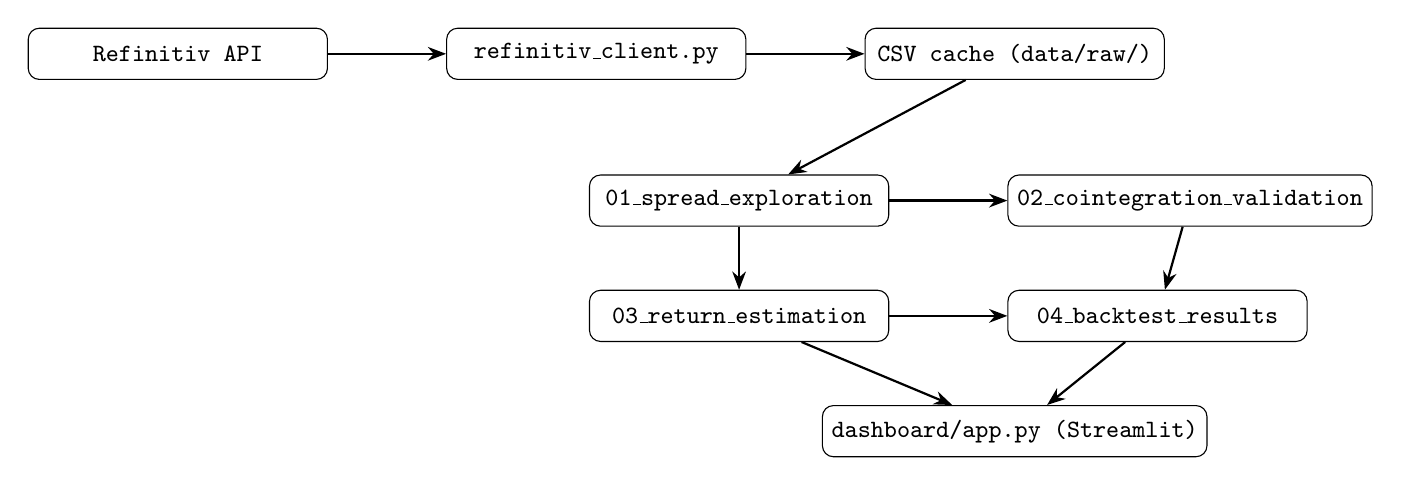
\begin{tikzpicture}[
  node distance=0.8cm and 1.5cm,
  box/.style={draw, rounded corners, minimum width=3.8cm, minimum height=0.65cm, align=center, font=\ttfamily\small},
  arr/.style={-{Stealth}, thick}
]

% Row 1: data ingestion
\node[box] (api)    {Refinitiv API};
\node[box, right=of api] (client) {refinitiv\_client.py};
\node[box, right=of client] (cache) {CSV cache (data/raw/)};

% Row 2: notebooks
\node[box, below=1.2cm of cache, xshift=-3.5cm] (nb01) {01\_spread\_exploration};
\node[box, right=of nb01] (nb02) {02\_cointegration\_validation};

% Row 3: notebooks
\node[box, below=0.8cm of nb01] (nb03) {03\_return\_estimation};
\node[box, right=of nb03] (nb04) {04\_backtest\_results};

% Row 4: dashboard
\node[box, below=0.8cm of nb03, xshift=3.5cm] (dash) {dashboard/app.py (Streamlit)};

% Arrows
\draw[arr] (api)    -- (client);
\draw[arr] (client) -- (cache);
\draw[arr] (cache)  -- (nb01);
\draw[arr] (nb01)   -- (nb02);
\draw[arr] (nb01)   -- (nb03);
\draw[arr] (nb02)   -- (nb04);
\draw[arr] (nb03)   -- (nb04);
\draw[arr] (nb03)   -- (dash);
\draw[arr] (nb04)   -- (dash);

\end{tikzpicture}
\caption{Data flow through the four-notebook pipeline and dashboard.}
\label{fig:pipeline}
\end{figure}

\subsection{Data Ingestion and Caching}

Price data are retrieved from the LSEG Refinitiv Workspace API via a custom client (\texttt{src/data/refinitiv\_client.py}). The client implements an incremental caching strategy: on first request, the full date range is fetched and persisted as a CSV file in \texttt{data/raw/}. Subsequent requests check the cache and only fetch the date gaps not yet covered, merging new data with the existing cache. Cache keys are derived from a hash of the ticker list, interval, and field set, ensuring deterministic file naming regardless of request order. This design minimises API calls during iterative development while guaranteeing reproducibility.

The client also handles column normalisation (mapping LSEG field codes such as \texttt{TRDPRC\_1} to \texttt{Close}), forward-filling of up to five consecutive missing values, and automatic dropping of columns with more than 10\% missing data. S\&P~500 benchmark prices are sourced separately via the \texttt{yfinance} library.

\section{Spread Exploration}

The first notebook (\texttt{01\_spread\_exploration}) loads in-sample close prices for all 26 universe constituents and constructs the 16 candidate spreads using the OLS hedge ratios. For each pair, it produces:
\begin{itemize}
    \item Normalised price overlays to visualise co-movement.
    \item Spread level and distribution plots.
    \item Rolling half-life and Hurst exponent time series.
    \item Rolling $z$-score plots with entry/exit threshold annotations.
\end{itemize}

These are implemented in the \texttt{spread\_analysis} module, which provides functions \texttt{compute\_spread()}, \texttt{compute\_half\_life()}, \texttt{compute\_hurst\_exponent()}, and \texttt{compute\_zscore()}. The half-life function fits the AR(1) regression (Equation~\ref{eq:ar1}) using ordinary least squares and returns the half-life in trading days. The Hurst exponent function computes the variogram across lags up to \texttt{max\_lag} (default: 100) and estimates $H$ via log-log regression on $\log(\tau_\ell)$ against $\log(\ell)$. Diagnostics are aggregated in the notebook into a summary DataFrame for tabular comparison across pairs.

\section{Cointegration Validation}

The second notebook (\texttt{02\_cointegration\_validation}) applies the full Engle--Granger screening pipeline to all 16 candidate pairs on the in-sample data, then assesses out-of-sample stability.

\subsection{Screening Implementation}

The \texttt{cointegration} module implements the screening procedure as follows:
\begin{itemize}
    \item \texttt{adf\_test(series)} applies the Augmented Dickey--Fuller test using the \texttt{statsmodels} implementation with automatic AIC-based lag selection. It returns the test statistic, $p$-value, number of lags, and critical values.
    \item \texttt{engle\_granger\_test(y, x)} performs the two-step procedure: it fits the OLS cointegrating regression, extracts residuals, and applies the ADF test to the residuals. Both orderings ($y$ on $x$ and $x$ on $y$) are tested, and the ordering with the lower residual $p$-value is retained. The function returns the hedge ratio $\hat{\beta}$, intercept $\hat{\alpha}$, ADF statistic, $p$-value, and the selected ordering.
    \item \texttt{screen\_pairs(prices, pairs)} iterates over all candidate pairs, verifies that both legs are $I(1)$, runs the Engle--Granger test, and returns a DataFrame of results with a boolean \texttt{cointegrated} column (true if $p < 0.05$).
\end{itemize}

\subsection{Out-of-Sample Stability}

To assess whether in-sample cointegration relationships persist, the notebook re-estimates the cointegrating regression on the OOS period and compares hedge ratios, ADF statistics, and spread dynamics. Rolling half-life plots spanning both periods provide visual confirmation of parameter stability. This validation step informs which pairs are included in the final portfolio.

Two additional formal tests are also implemented. The \textbf{KPSS test} (\texttt{statsmodels.tsa.stattools.kpss}) complements ADF by reversing the null hypothesis: stationarity is accepted only when ADF rejects non-stationarity \emph{and} KPSS fails to reject stationarity. The \textbf{Chow test} formally tests whether the cointegrating regression coefficients $(\hat{\beta}, \hat{\alpha})$ are stable across the IS/OOS split by comparing the pooled residual sum of squares against the sum from separate IS and OOS regressions, yielding an $F$-statistic under $H_0$: no structural break.

\section{Return Estimation}

The third notebook (\texttt{03\_return\_estimation}) computes expected returns under both the OU-implied and historical mean approaches.

The \texttt{return\_estimation} module provides:
\begin{itemize}
    \item \texttt{compute\_spread\_returns(y\_prices, x\_prices, hedge\_ratio)} --- computes daily log spread returns as $\ln(Y_t/Y_{t-1}) - \beta \cdot \ln(X_t/X_{t-1})$.
    \item \texttt{build\_spread\_return\_matrix(prices, coint\_pairs)} --- constructs the full $T \times n$ matrix of spread returns for all cointegrated pairs.
    \item \texttt{ou\_implied\_spread\_return(spread, half\_life)} --- implements Equation~\ref{eq:ou_expected_return}, computing $\kappa = \ln 2 / h$ and the conditional expected spread change.
    \item \texttt{build\_ou\_implied\_returns(prices, coint\_pairs)} --- applies the OU-implied estimator to all pairs and returns an annualised expected return vector.
    \item \texttt{historical\_mean\_return(returns)} --- computes the sample mean, optionally over a trailing window.
    \item \texttt{shrinkage\_covariance(returns)} --- estimates the covariance matrix using the Ledoit--Wolf shrinkage estimator from \texttt{scikit-learn}, which shrinks the sample covariance towards a scaled identity target.
\end{itemize}

The notebook produces a grouped bar chart comparing OU-implied, historical mean, and EWMA return estimates across pairs, along with a correlation heatmap of spread returns to visualise diversification potential.

\section{Portfolio Optimisation Module}

The \texttt{optimiser} module implements the Markowitz mean-variance framework in spread space.

\begin{itemize}
    \item \texttt{minimum\_variance\_weights(returns, cov\_matrix, l2\_reg)} --- solves the minimum-variance problem (Equation~\ref{eq:min_var}) using Sequential Least Squares Programming (SLSQP) from \texttt{scipy.optimize}. The long-only constraint ($w_i \geq 0$) and full-investment constraint ($\sum w_i = 1$) are enforced explicitly. The optional $L_2$ regularisation term \texttt{l2\_reg}$\cdot \|\mathbf{w}\|_2^2$ is added to the objective to improve numerical stability and reduce weight concentration.
    \item \texttt{maximum\_sharpe\_weights(returns, expected\_returns, cov\_matrix, rf\_annual)} --- solves the maximum Sharpe ratio problem (Equation~\ref{eq:max_sharpe}) by minimising the negative Sharpe ratio subject to the same long-only and full-investment constraints. Custom expected returns (e.g.\ OU-implied) can be passed via \texttt{expected\_returns}; if omitted, the historical sample mean is used.
    \item \texttt{compute\_efficient\_frontier(returns, expected\_returns, cov\_matrix, n\_points, rf\_annual)} --- generates the efficient frontier by solving the minimum-variance problem for a range of target returns, anchored between the global minimum-variance portfolio return and the maximum single-asset expected return.
\end{itemize}

Return and volatility figures are annualised from daily values. Log-return expected returns are converted to annualised arithmetic returns via $\mu_{\text{ann}} = \mathrm{expm1}(252 \cdot \mu_{\text{daily}})$, i.e.\ $\exp(252\,\mu_{\text{daily}}) - 1$, which correctly compounds the daily log return. Volatilities are scaled as $\sigma_{\text{ann}} = \sigma_{\text{daily}} \cdot \sqrt{252}$. The optimiser accepts either OU-implied or historical expected returns, enabling direct comparison of the resulting allocations.

\section{Backtesting Engine}

The backtesting engine (\texttt{src/backtesting/engine.py}) simulates pair-level trading and computes performance metrics.

\subsection{Architecture}

The engine uses a dataclass-based configuration pattern:
\begin{itemize}
    \item \texttt{BacktestConfig} stores all strategy parameters (entry, exit, and stop-loss $z$-score thresholds, lookback window, transaction cost rate, and initial capital) with validation in \texttt{\_\_post\_init\_\_} to enforce $z_{\text{exit}} < z_{\text{entry}} < z_{\text{stop}}$.
    \item \texttt{BacktestResult} is a container holding daily returns, cumulative returns, position history, trade log, summary metrics, spread, and $z$-score series.
    \item \texttt{PairsBacktestEngine} orchestrates the full pipeline: spread and $z$-score computation, signal generation, PnL calculation, trade logging, and metric aggregation.
\end{itemize}

\subsection{Signal Generation}

The signal generator implements the $z$-score state machine described in Section~\ref{sec:backtesting}. It iterates sequentially through the $z$-score series, maintaining a position state variable that transitions between $\{-1, 0, +1\}$ based on threshold crossings. The sequential iteration is necessary because the position on day $t$ depends on the position on day $t-1$, precluding vectorised computation.

\subsection{PnL and Transaction Costs}

The PnL computation deploys the full initial capital into each active position. On each day, the number of spread units is recalculated as $n_t = C_0 / (Y_t + |\beta| X_t)$ to reflect changing notional values. The dollar PnL is $\text{pos}_{t-1} \cdot n_{t-1} \cdot (\Delta Y_t - \beta \cdot \Delta X_t)$, from which transaction costs (proportional to the absolute position change) are deducted.

\subsection{Metrics and Benchmarks}

The \texttt{metrics} module provides three core functions: \texttt{compute\_ex\_post\_sharpe\_ratio()}, \texttt{compute\_max\_drawdown()}, and \texttt{compute\_volatility\_reduction()}, each implemented as described in Section~\ref{sec:backtesting}. The \texttt{benchmarks} module constructs comparison return series: a constant risk-free rate, equal-weight buy-and-hold of all universe constituents, per-pair buy-and-hold of both legs, and the S\&P~500 index. A \texttt{historical\_mpt\_returns()} function computes the out-of-sample returns of a traditional max-Sharpe portfolio estimated on in-sample asset returns, serving as the primary baseline for comparison.

Three statistical tests are implemented in the fourth notebook to strengthen the empirical evaluation:
\begin{itemize}
    \item \textbf{Bootstrap confidence intervals} (10{,}000 resamples) on the annualised Sharpe ratio for each strategy, quantifying sampling uncertainty over the short OOS window.
    \item \textbf{Paired $t$-test and Wilcoxon signed-rank test} comparing OU Max-Sharpe against Historical Max-Sharpe daily returns, directly testing whether the observed Sharpe difference is statistically significant.
    \item \textbf{Sensitivity analysis}: a grid sweep over entry $z$-score thresholds $\{1.5, 2.0, 2.5, 3.0\}$ and transaction costs $\{0, 5, 10, 20, 30\}$ bps, assessing the robustness of per-pair backtest results to parameter choice.
    \item \textbf{Leave-one-pair-out (LOPO) robustness}: each pair is removed in turn, the OU Max-Sharpe portfolio is re-optimised on the remaining spreads, and OOS Sharpe is recomputed, testing whether the portfolio result is driven by a single spread.
\end{itemize}

\section{Dashboard Interface}

An interactive Streamlit dashboard (\texttt{src/dashboard/app.py}) provides a user-facing interface for exploring the full pipeline. The dashboard enables users to:
\begin{itemize}
    \item Select candidate pairs and configure date ranges and capital.
    \item View cointegration screening results (horizontal bar chart of $p$-values with significance threshold).
    \item Inspect spread dynamics: spread with $\pm 2\sigma$ Bollinger bands, $z$-score with entry/exit thresholds, and position timelines.
    \item Compare return estimation methods via grouped bar charts and rolling estimate plots.
    \item Run backtests and view cumulative return plots, drawdown charts, return distribution histograms, and rolling Sharpe ratios.
    \item Visualise the efficient frontier with annotated max-Sharpe and min-variance portfolios.
    \item Compare strategy performance against all benchmarks in a unified cumulative return chart with a metrics summary table.
\end{itemize}

The visualisation layer is implemented in a separate \texttt{components.py} module using Plotly, which provides interactive zoom, hover tooltips, and export capabilities. Chart functions are stateless and accept data as arguments, ensuring they are reusable across the notebooks and the dashboard.

\section{Summary}

This chapter has described the implementation of the pairs-trading portfolio optimisation system. The codebase is organised into a four-notebook analysis pipeline supported by three library packages (\texttt{modelling}, \texttt{backtesting}, \texttt{data}) and an interactive Streamlit dashboard. Key design decisions include incremental data caching for API efficiency, a clean modular API for testability, dataclass-based configuration for the backtesting engine, and separation of visualisation logic into reusable Plotly chart components. Chapter~\ref{chap:results} presents the empirical results produced by this implementation.

\chapter{Testing and Results}
\label{chap:results}
\section{Cointegration Screening}

\begin{table}[htbp]
\centering
\caption{Engle-Granger Cointegration Screening Results (16 candidate pairs, in-sample: Jan 2019 -- Dec 2023)}
\label{tab:cointegration_screening}
\resizebox{\textwidth}{!}{%
\begin{tabular}{l l c c c c c c c}
\toprule
Dependent & Independent & Hedge Ratio ($\hat{\beta}$) & Intercept ($\hat{\alpha}$) & ADF Stat & $p$-value & $y$ is $I(1)$ & $x$ is $I(1)$ & Cointegrated \\
\midrule
GS.N    & MS.N    &  0.780 &  2.351 & $-$3.667 & 0.020 & Yes & Yes & \textbf{Yes} \\
KO.N    & PEP.O   &  0.641 &  0.789 & $-$3.470 & 0.035 & Yes & Yes & \textbf{Yes} \\
DAL.N   & UAL.O   &  0.672 &  1.068 & $-$3.460 & 0.036 & Yes & Yes & \textbf{Yes} \\
CVX.N   & XOM.N   &  0.698 &  1.813 & $-$3.234 & 0.064 & Yes & Yes & No \\
AMZN.O  & GOOGL.O &  0.630 &  1.942 & $-$2.442 & 0.305 & Yes & Yes & No \\
HAL.N   & SLB.N   &  0.997 & $-$0.344 & $-$2.370 & 0.339 & Yes & Yes & No \\
AMD.O   & NVDA.O  &  0.811 &  1.999 & $-$2.310 & 0.368 & Yes & Yes & No \\
AMZN.O  & MSFT.O  &  0.516 &  2.027 & $-$2.141 & 0.455 & Yes & Yes & No \\
MRK.N   & ABBV.N  &  0.431 &  2.366 & $-$1.980 & 0.539 & Yes & Yes & No \\
INTC.O  & AMD.O   & $-$0.081 & 4.154 & $-$1.958 & 0.550 & Yes & Yes & No \\
JNJ.N   & PFE.N   &  0.423 &  3.466 & $-$1.908 & 0.576 & Yes & Yes & No \\
INTC.O  & TSM.N   & $-$0.087 & 4.201 & $-$1.890 & 0.585 & Yes & Yes & No \\
META.O  & GOOGL.O &  0.543 &  2.953 & $-$1.681 & 0.685 & Yes & Yes & No \\
TSM.N   & NVDA.O  &  0.476 &  3.071 & $-$1.340 & 0.817 & Yes & Yes & No \\
BAC.N   & JPM.N   &  0.854 & $-$0.666 & $-$1.230 & 0.850 & Yes & Yes & No \\
TGT.N   & COST.O  &  0.856 & $-$0.125 & $-$0.869 & 0.925 & Yes & Yes & No \\
\bottomrule
\end{tabular}%
}% end resizebox
\par\smallskip
\begin{minipage}{\textwidth}
\small
Dep./Indep.: Dependent/Independent variable in the cointegrating regression $Y_t = \hat{\alpha} + \hat{\beta} X_t + \epsilon_t$.
$\hat{\beta}$: hedge ratio; $\hat{\alpha}$: intercept. ADF Stat and $p$-val: residual ADF test statistic and MacKinnon (2010) $p$-value.
$y{:}I(1)$, $x{:}I(1)$: whether each leg passes the unit root filter. Coint.: cointegrated at 5\% significance ($p < 0.05$).
Source: Author's calculations on \texttt{01\_spread\_exploration.ipynb}.

\end{minipage}
\end{table}

\section{Spread Characterisation}

Based on the results in Table~\ref{tab:cointegration_screening}, two pairs were confirmed cointegrated at the 5\% significance level: GS.N/MS.N and KO.N/PEP.O. CVX.N/XOM.N was borderline ($p = 0.064$) and excluded. Spreads for each confirmed pair are computed as the OLS residual $S_t = \ln P^y_t - \hat{\beta}\ln P^x_t - \hat{\alpha}$ and characterised by their half-life, Hurst exponent, z-score, and spread statistics.

Table~\ref{tab:spread_characterisation} and Figures~\ref{fig:normalised_prices}
present the spread characterisation results for the two cointegrated pairs.

\begin{table}[htbp]
\centering
\caption{Spread Characterisation Summary --- Cointegrated Pairs (In-Sample: Jan 2019 -- Dec 2023)}
\label{tab:spread_characterisation}
\resizebox{\textwidth}{!}{%
\begin{tabular}{l l c c c c c c c}
\toprule
Dep. & Indep. & Half-Life & Hurst & $z$-Score & $\mu_S$ & $\sigma_S$ & ADF Stat & ADF $p$ \\
 & & (days) & Exp. & (current) & & & & \\
\midrule
GS.N  & MS.N  & 41.8 & 0.403 & 0.675 & 0.000 & 0.056 & $-$3.666 & 0.005 \\
KO.N  & PEP.O & 40.3 & 0.421 & 0.809 & 0.000 & 0.047 & $-$3.469 & 0.009 \\
DAL.N & UAL.O & 52.9 & 0.414 & 1.315 & 0.000 & 0.076 & $-$3.459 & 0.009 \\
\bottomrule
\end{tabular}%
}
\par\smallskip
\begin{minipage}{\textwidth}
\small
Dep.: Dependent leg; Indep.: Independent leg of the cointegrating regression. 
$\mu_S$: spread mean; $\sigma_S$: spread standard deviation; ADF Stat/ADF $p$: residual ADF test statistic and MacKinnon (2010) $p$-value on the spread.\\
Half-life estimated via AR(1)/OU regression: $\kappa = \ln(2)/\text{half-life}$ gives $\kappa \approx 0.0166$ (GS/MS), $0.0172$ (KO/PEP), and $0.0131$ (DAL/UAL).\\
Hurst exponent $H < 0.5$ indicates mean-reverting (anti-persistent) dynamics. $z$-score uses 60-day rolling window at end of training period.\\
Spread mean $\mu_S = 0$ by construction (demeaned OLS residuals). Source: Author's calculations on \texttt{01\_spread\_exploration.ipynb}.
\end{minipage}

\end{table}

\begin{figure}[htbp]
    \centering
    
\includegraphics[width=\textwidth]{figures/01_normalised_prices.pdf}
    \caption{Normalised log price series for the three cointegrated pairs over
    the in-sample period (January 2019 -- December 2023). Each series is
    normalised to zero at the start of the sample period to highlight co-movement.
    (a)~GS/MS (Financials); (b)~KO/PEP (Consumer Staples);(c)~DAL/UAL (Airlines).}
    \label{fig:normalised_prices}
\end{figure}

\begin{figure}[htbp]
    \centering
    
\includegraphics[width=\textwidth]{figures/01_spread_characterisation.pdf}
    \caption{Spread characterisation summary for the two cointegrated pairs
    (January 2019 -- December 2023).
    (a) Half-life of mean reversion in trading days; dashed line marks the 60-day threshold.
    (b) Hurst exponent; dashed line marks the random walk boundary of 0.5.
    (c) Current $z$-score at the end of the training window; dotted lines mark $\pm2\sigma$.
    (d) ADF $p$-value on the spread; dashed line marks the 5\% significance level.
    Hatched bars indicate pairs that fail the respective threshold.}
    \label{fig:spread_characterisation}
\end{figure}

\begin{figure}[htbp]
    \centering
    
\includegraphics[width=0.9\textwidth]{figures/01_spread_levels.pdf}
    \caption{Spread levels with $\pm1\sigma$ and $\pm2\sigma$ bands for each
    cointegrated pair over the in-sample period (January 2019 -- December 2023).
    The spread is defined as $S_t = \ln P^y_t - \hat{\beta}\ln P^x_t - \hat{\alpha}$.
    (a)~KO/PEP; (b)~GS/MS; (c)~DAL/UAL.}
    \label{fig:spread_levels}
\end{figure}

\begin{figure}[htbp]
    \centering
    
\includegraphics[width=0.9\textwidth]{figures/01_spread_zscores.pdf}
    \caption{Rolling $z$-scores (60-day window) for the two cointegrated pairs
    over the in-sample period (January 2019 -- December 2023). Dotted lines mark
    the $\pm2\sigma$ entry thresholds. The $z$-score at the end of the training
    window feeds directly into the OU-implied return estimation.
    (a)~KO/PEP; (b)~GS/MS; (c)~DAL/UAL.}
    \label{fig:spread_zscores}
\end{figure}

\begin{figure}[htbp]
    \centering
    
\includegraphics[width=0.9\textwidth]{figures/01_spread_rolling_halflife.pdf}
    \caption{Rolling half-life of mean reversion (252-day window, EWM 21-day smoothed).
    Dashed line denotes the 60-day tradeability threshold.
    Shaded regions indicate periods where the smoothed half-life exceeded the threshold.
    (a)~KO/PEP; (b)~GS/MS; (c)~DAL/UAL.}
    \label{fig:spread_rolling_halflife}
\end{figure}

\FloatBarrier

\section{Cointegration Validation}

Out-of-sample spreads are constructed using hedge ratios and intercepts
estimated solely on the in-sample period, ensuring no forward-looking
information is incorporated. Table~\ref{tab:oos_spread_stats} presents
the distributional shift in each spread across the IS and OOS periods,
while Table~\ref{tab:cointegration_validation} reports the formal
statistical test results. Figure~\ref{fig:oos_eg_pvalues} presents
the full IS vs OOS Engle-Granger $p$-value comparison across all
nine candidate pairs.

\begin{table}[htbp]
\centering
\caption{Spread statistics across in-sample (IS: January 2019 -- December 2023) and out-of-sample (OOS: January 2024 -- December 2025) periods, constructed using in-sample hedge ratios.\\}
\label{tab:oos_spread_stats}
\begin{tabular}{lcccccccc}
\toprule
& \multicolumn{2}{c}{Mean} & \multicolumn{2}{c}{Std Dev} & \multicolumn{2}{c}{Min} & \multicolumn{2}{c}{Max} \\
\cmidrule(lr){2-3} \cmidrule(lr){4-5} \cmidrule(lr){6-7} \cmidrule(lr){8-9}
Pair & IS & OOS & IS & OOS & IS & OOS & IS & OOS \\
\midrule
GS/MS   & 0.000 & $+$0.250 & 0.056 & 0.082 & $-$0.145 & $+$0.067 & $+$0.110 & $+$0.411 \\
KO/PEP  & 0.000 & $+$0.170 & 0.047 & 0.110 & $-$0.173 & $-$0.016 & $+$0.111 & $+$0.367 \\
DAL/UAL & 0.000 & $+$0.026 & 0.076 & 0.119 & $-$0.201 & $-$0.199 & $+$0.175 & $+$0.280 \\
\bottomrule
\end{tabular}

\par\smallskip
\begin{minipage}{15cm}
\small
The GS/MS OOS minimum (+0.067) exceeds the IS mean (0.000), indicating the spread never reverted to its historical equilibrium during the OOS period. \\
Source: Author's calculations on \texttt{02\_cointegration\_validation.ipynb}.
\end{minipage}
\end{table}


\begin{table}[htbp]
\centering
\caption{Cointegration validation statistics across IS (January 2019 -- December 2023) and OOS (January 2024 -- December 2025) periods. ADF $p$-values below 0.05 indicate spread stationarity at the 5\% significance level. Half-life below 60 trading days and Hurst exponent below 0.5 indicate mean reversion.\\}
\label{tab:cointegration_validation}
\begin{tabular}{lccccccc}
\toprule
& \multicolumn{2}{c}{ADF $p$-value}
& \multicolumn{2}{c}{Half-Life (days)}
& \multicolumn{2}{c}{Hurst Exponent}
& OOS \\
\cmidrule(lr){2-3} \cmidrule(lr){4-5} \cmidrule(lr){6-7}
Pair & IS & OOS & IS & OOS & IS & OOS & $z$-score \\
\midrule
GS/MS   & 0.005 & 0.452 & 41.8 &  81.1 & 0.403 & 0.362 & 1.015 \\
KO/PEP  & 0.009 & 0.622 & 40.3 & 156.4 & 0.421 & 0.575 & 0.604 \\
DAL/UAL & 0.009 & 0.583 & 52.9 & 103.1 & 0.414 & 0.421 & 0.872 \\
\bottomrule
\end{tabular}

\par\smallskip
\begin{minipage}{15cm}
\small
Neither spread remains stationary OOS using IS hedge ratios. KO/PEP Hurst crosses above 0.5, indicating transition to near-random-walk behaviour.\\
Source: Author's calculations on \texttt{02\_cointegration\_validation.ipynb}.
\end{minipage}
\end{table}

\begin{figure}[htbp]
    \centering
    
\includegraphics[width=\textwidth]{figures/02_oos_eg_pvalues.pdf}
    \caption{IS vs OOS Engle-Granger $p$-values for all 16 sector-candidate pairs.
    Panel labels (a)--(p) correspond to the pairs listed in Table~\ref{tab:cointegration_screening}.
    Hatched bars indicate pairs that fail the 5\% significance threshold.
    Of the three pairs that pass IS screening, GS/MS and KO/PEP remain the most stable OOS;
    DAL/UAL degrades substantially. The remaining 13 pairs show no evidence of cointegration
    in either period.}
    \label{fig:oos_eg_pvalues}
\end{figure}

\begin{figure}[htbp]
    \centering
    
\includegraphics[width=\textwidth]{figures/02_spread_is_oos_concat.pdf}
    \caption{Spread levels across the full sample period (January 2019 --
    December 2025). The dashed vertical line marks the IS/OOS boundary
    (January 2024). Horizontal lines and shading denote IS $\pm1\sigma$
    and $\pm2\sigma$ bands; persistent OOS displacement beyond these bounds
    indicates a structural break in the cointegrating relationship.
    (a)~KO/PEP; (b)~GS/MS; (c)~DAL/UAL.}
    \label{fig:spread_is_oos_concat}
\end{figure}

\begin{figure}[htbp]
    \centering
    
\includegraphics[width=\textwidth]{figures/02_zscore_is_oos.pdf}
    \caption{Rolling 60-day $z$-score across the full sample period
    (January 2019 -- December 2025). The dashed vertical line marks the
    IS/OOS boundary. Shaded regions indicate $|z|>2\sigma$ exceedances.
    Persistent non-zero $z$-scores in the OOS period are consistent with
    a shift in the spread equilibrium level.
    (a)~KO/PEP; (b)~GS/MS; (c)~DAL/UAL.}
    \label{fig:zscore_is_oos}
\end{figure}

\begin{figure}[htbp]
    \centering
    
\includegraphics[width=\textwidth]{figures/02_rolling_halflife_is_oos.pdf}
    \caption{Rolling half-life of mean reversion across the full sample
    period (January 2019 -- December 2025). Faint lines show raw estimates;
    bold lines show 21-day exponentially weighted smoothed values. The dashed
    horizontal line marks the 60-day tradability threshold. The dashed vertical
    line marks the IS/OOS boundary.
    (a)~KO/PEP; (b)~GS/MS; (c)~DAL/UAL.}
    \label{fig:rolling_halflife_is_oos}
\end{figure}

\begin{table}[htbp]
\centering
\caption{IS vs OOS Engle-Granger $p$-values and hedge ratio drift across all 16 candidate pairs.
Sorted by IS $p$-value. Hedge ratio drift = $|\hat{\beta}_{\text{OOS}} - \hat{\beta}_{\text{IS}}|$.}
\label{tab:cointegration_comparison}
\resizebox{\linewidth}{!}{%
\begin{tabular}{l cc cc c cc}
\toprule
& \multicolumn{2}{c}{EG $p$-value} & \multicolumn{2}{c}{Hedge Ratio $\hat{\beta}$} & Drift & \multicolumn{2}{c}{Cointegrated} \\
\cmidrule(lr){2-3} \cmidrule(lr){4-5} \cmidrule(lr){7-8}
Pair & IS & OOS & IS & OOS & $|\Delta\hat{\beta}|$ & IS & OOS \\
\midrule
GS.N/MS.N      & \textbf{0.020} & \textbf{0.019} &  0.780 &  1.120 & 0.340 & \textbf{Yes} & \textbf{Yes} \\
KO.N/PEP.O    & \textbf{0.035} & 0.224          &  0.641 & $-$0.350 & 0.991 & \textbf{Yes} & No \\
DAL.N/UAL.O   & \textbf{0.036} & 0.621          &  0.672 &  0.429 & 0.242 & \textbf{Yes} & No \\
CVX.N/XOM.N   & 0.064          & 0.118          &  0.698 &  0.470 & 0.228 & No & No \\
AMZN.O/GOOGL.O & 0.305         & 0.185          &  0.630 &  0.440 & 0.190 & No & No \\
SLB.N/HAL.N   & 0.339          & 0.242          &  0.997 &  0.676 & 0.321 & No & No \\
NVDA.O/AMD.O  & 0.368          & 0.060          &  0.811 &  0.293 & 0.518 & No & No \\
AMZN.O/MSFT.O & 0.455          & 0.265          &  0.516 &  0.897 & 0.382 & No & No \\
MRK.N/ABBV.N  & 0.539          & 0.507          &  0.431 & $-$0.318 & 0.749 & No & No \\
INTC.O/AMD.O  & 0.550          & 0.076          & $-$0.081 & 0.831 & 0.912 & No & No \\
JNJ.N/PFE.N   & 0.576          & 0.182          &  0.423 & $-$0.166 & 0.589 & No & No \\
INTC.O/TSM.N  & 0.585          & 0.731          & $-$0.087 & $-$0.212 & 0.124 & No & No \\
META.O/GOOGL.O & 0.685         & 0.290          &  0.543 &  0.525 & 0.018 & No & No \\
NVDA.O/TSM.N  & 0.817          & 0.012          &  0.476 &  1.120 & 0.644 & No & No$^{\dagger}$ \\
BAC.N/JPM.N   & 0.850          & 0.384          &  0.854 &  0.697 & 0.157 & No & No \\
TGT.N/COST.O  & 0.925          & 0.162          &  0.856 & $-$0.318 & 1.174 & No & No \\
\bottomrule
\end{tabular}%
}% end resizebox

\par\smallskip
\begin{minipage}{15cm}
\small
$^{\dagger}$NVDA/TSM: OOS $p$-value passes threshold but $y$ fails $I(1)$ test --- cointegration requires both series to be $I(1)$.\\
KO/PEP hedge ratio sign reversal ($+0.641 \to -0.350$) and DAL/UAL OOS $p$-value surge indicate structural breaks in the cointegrating relationship.\\
Source: Author's calculations on \texttt{02\_cointegration\_validation.ipynb}.
\end{minipage}
\end{table}

\FloatBarrier

\subsection{KPSS Complement and Chow Structural Break Tests}

Table~\ref{tab:kpss_results} applies the KPSS test alongside ADF on both IS and OOS spreads.
The KPSS null hypothesis is stationarity (the reverse of ADF), so mean reversion is only
confirmed when ADF rejects non-stationarity \emph{and} KPSS fails to reject stationarity.

\begin{table}[htbp]
\centering
\caption{ADF and KPSS stationarity tests on IS and OOS spreads (using IS hedge ratios).
Mean-reversion (MR) consensus requires ADF $p < 0.05$ and KPSS $p > 0.05$ simultaneously.}
\label{tab:kpss_results}
\resizebox{\textwidth}{!}{%
\begin{tabular}{lcccccc}
\toprule
& \multicolumn{3}{c}{In-Sample (2019--2023)} & \multicolumn{3}{c}{Out-of-Sample (2024--2025)} \\
\cmidrule(lr){2-4} \cmidrule(lr){5-7}
Pair & ADF $p$ & KPSS $p$ & MR Consensus & ADF $p$ & KPSS $p$ & MR Consensus \\
\midrule
GS.N/MS.N   & 0.005 & 0.019 & No  & 0.452 & 0.010 & No \\
KO.N/PEP.O  & 0.009 & 0.100 & Yes & 0.622 & 0.010 & No \\
DAL.N/UAL.O & 0.009 & 0.080 & Yes & 0.584 & 0.010 & No \\
\bottomrule
\multicolumn{7}{l}{\small KPSS $p$-value of 0.010 denotes the tabulated lower bound (i.e.\ $p \leq 0.010$); null of stationarity is strongly rejected.} \\
\multicolumn{7}{l}{\small IS consensus: KO/PEP and DAL/UAL achieve consensus; GS/MS fails KPSS despite low ADF $p$, indicating non-stationarity is borderline.} \\
\multicolumn{7}{l}{\small OOS: All three pairs lose the MR consensus, consistent with Table~\ref{tab:cointegration_validation}.} \\
\multicolumn{7}{l}{\small Source: Author's calculations on \texttt{02\_cointegration\_validation.ipynb}.}
\end{tabular}%
}
\end{table}

Table~\ref{tab:chow_results} presents the Chow test for structural break in the cointegrating
regression across the IS/OOS split. The null hypothesis is that the regression coefficients
$(\hat{\beta}, \hat{\alpha})$ are identical in both periods.

\begin{table}[htbp]
\centering
\caption{Chow test for structural break in the cointegrating regression $y = \alpha + \beta x$
across the IS/OOS split (IS: 2019--2023; OOS: 2024--2025).
H$_0$: no structural break (regression coefficients are equal in both periods).}
\label{tab:chow_results}
\begin{tabular}{lrrcl}
\toprule
Pair & $F$-statistic & $p$-value & df & Conclusion \\
\midrule
GS.N/MS.N   & 2406.3 & $<0.001$ & (2, 2007) & Structural break detected \\
KO.N/PEP.O  & 3078.4 & $<0.001$ & (2, 2007) & Structural break detected \\
DAL.N/UAL.O &  269.5 & $<0.001$ & (2, 2007) & Structural break detected \\
\bottomrule
\multicolumn{5}{l}{\small The $F$-statistic compares the residual sum of squares of separate IS and OOS regressions} \\
\multicolumn{5}{l}{\small against the pooled regression. All three pairs strongly reject the null at any conventional} \\
\multicolumn{5}{l}{\small significance level, confirming that the cointegrating relationship is not stable over time.} \\
\multicolumn{5}{l}{\small Source: Author's calculations on \texttt{02\_cointegration\_validation.ipynb}.}
\end{tabular}
\end{table}

\FloatBarrier

\section{Return Estimation}

OU-implied expected returns are derived from the end-of-IS $z$-score for each
confirmed pair. A positive $z$-score (spread above mean) implies the spread is
expected to fall, producing a negative OU-implied return; a negative $z$-score
implies the spread is expected to rise, producing a positive return.
Table~\ref{tab:return_estimation} presents the sanity check confirming directional
consistency between the $z$-score and OU-implied return signal.

\begin{table}[htbp]
\centering
\caption{End-of-sample $z$-score validation and OU-implied expected returns (IS period: Jan 2019 -- Dec 2023)}
\label{tab:return_estimation}
\resizebox{\textwidth}{!}{%
\begin{tabular}{lrrrll}
\toprule
Pair & End-of-IS $z$-Score & OU-Implied $\mu$ (ann.) & Historical $\mu$ (ann.) & Signal & Consistent \\
\midrule
GS/MS  & $+$1.739 & $-$10.69\% & GS: $+$11.9\%, MS: $+$15.5\% & Spread well above mean & Yes \\
KO/PEP & $-$0.759 & $+$1.93\%  & KO: $+$6.4\%,\ PEP: $+$8.3\% & Spread below mean      & Yes \\
\bottomrule
\multicolumn{6}{l}{\small OU-implied $\mu$ computed via rolling 60-day OU model, annualised at 252 trading days per year.} \\
\multicolumn{6}{l}{\small Historical $\mu$ is the annualised sample mean of daily returns over the IS period.} \\
\multicolumn{6}{l}{\small Source: Author's calculations on \texttt{03\_return\_estimation.ipynb}.}
\end{tabular}%
}
\end{table}

\begin{figure}[htbp]
    \centering
    
\includegraphics[width=\textwidth]{figures/03_cumulative_returns.pdf}
    \caption{Cumulative returns of each cointegrated spread versus its constituent
    assets over the in-sample period (January 2019 -- December 2023). All series
    are indexed to 1.0 at the start. The spread return reflects the daily change in
    the OLS residual $S_t = \ln P^y_t - \hat{\beta}\ln P^x_t - \hat{\alpha}$.}
    \label{fig:cumulative_returns_is}
\end{figure}

\begin{figure}[htbp]
    \centering
    
\includegraphics[width=\textwidth]{figures/03_mu_comparison.pdf}
    \caption{Expected return estimates (annualised, IS 2019--2023).
    (a)~OU-implied $\mu$ by pair: GS/MS has a large negative implied return
    (spread well above equilibrium at end of IS); KO/PEP has a small positive
    implied return (spread slightly below equilibrium).
    (b)~Historical mean $\mu$ by ticker: all four assets exhibit positive
    historical means, producing a very different allocation under mean-variance
    optimisation.}
    \label{fig:mu_comparison}
\end{figure}

\begin{figure}[htbp]
    \centering
    
\includegraphics[width=0.9\textwidth]{figures/03_correlation_heatmap.pdf}
    \caption{Asset return correlation matrix for the four constituent tickers
    (GS.N, KO.N, MS.N, PEP.O) estimated over the in-sample period
    (January 2019 -- December 2023) using Ledoit-Wolf shrinkage covariance.
    GS and MS exhibit the highest within-pair correlation, consistent with
    their financial sector co-movement.}
    \label{fig:correlation_heatmap}
\end{figure}

\FloatBarrier

\section{Backtesting Results}

\subsection{Portfolio-Level Performance}

Table~\ref{tab:backtest_results} reports out-of-sample portfolio performance metrics
over the test period (January 2024 -- December 2025). The OU-Implied MPT portfolio
operates in spread space (GS/MS, KO/PEP and DAL/UAL as assets) under minimum-variance
weights; the Historical MPT portfolio operates in asset space (GS.N, KO.N, MS.N, PEP.O, DAL.N, UAL.O) under minimum-variance weights with historical mean returns.

\begin{table}[htbp]
    \centering
    \caption{Out-of-sample portfolio performance metrics (test period: January 2024 -- December 2025). Vol.\ Reduction is relative to the equal-weight spread baseline; negative values indicate higher volatility. Beta ($\hat{\beta}$) estimated via OLS against daily S\&P 500 returns.}
    \label{tab:backtest_results}
    \resizebox{\textwidth}{!}{%
    \begin{tabular}{lrrrrrr}
    \toprule
     & \multicolumn{5}{c}{Performance} & \multicolumn{1}{c}{Market Exposure} \\
    \cmidrule(lr){2-6} \cmidrule(lr){7-7}
     & Sharpe Ratio & Max Drawdown & Total Return & Ann.\ Volatility & Vol.\ Reduction & $\hat{\beta}$ \\
    \midrule
    Equal-Weight Spreads     & 0.625 & $-$10.6\% & $+$16.3\%  &  9.7\% & ---       & 0.233 \\
    Spread Min-Var ($\mu=0$) & 0.720 & $-$9.5\%  & $+$17.8\%  &  9.2\% & $+$4.5\%  & 0.216 \\
    Spread Max-Sharpe (OU)   & 0.963 & $-$11.5\% & $+$34.8\%  & 14.6\% & $-$51.3\% & 0.318 \\
    Hist Min-Var             & 0.711 & $-$13.1\% & $+$24.3\%  & 13.9\% & $-$43.6\% & 0.429 \\
    Hist Max-Sharpe          & 0.868 & $-$20.0\% & $+$38.8\%  & 18.7\% & $-$93.4\% & 0.785 \\
    Buy \& Hold (All Pairs) & 1.245 & $-$27.8\% & $+$74.0\% & 22.9\% & ---       & 1.040 \\
    S\&P 500 (SPY)           & 1.110 & $-$18.9\% & $+$44.3\%  & 16.0\% & ---       & 1.000 \\
    \bottomrule
    \multicolumn{7}{l}{\small Spread Min-Var ($\mu=0$) assumes zero expected returns; min-var objective is return-agnostic. Risk-free rate: 2\% p.a.} \\
    \multicolumn{7}{l}{\small Spread Min-Var weights: $\mathbf{w} = [0.35, 0.36, 0.29]$ (GS/MS, KO/PEP, DAL/UAL). Spread Max-Sharpe (OU): $w_{\text{GS/MS}} = 1.0$.} \\
    \multicolumn{7}{l}{\small Source: Author's calculations on \texttt{04\_backtest\_results.ipynb}.}
    \end{tabular}%
    }
\end{table}

\subsection{Per-Pair Mean-Reversion Backtest}

\begin{table}[htbp]
    \centering
    \caption{Per-pair $z$-score mean-reversion backtest metrics (OOS: January 2024 -- December 2025). Entry at $\pm2.0\sigma$, exit at $\pm0.5\sigma$.}
    \label{tab:perpair_backtest}
    \resizebox{\textwidth}{!}{%
    \begin{tabular}{lrrrrrrrr}
    \toprule
    Pair & Sharpe & Max DD & Total Return & Ann.\ Vol & Trades & Days in Position & Win Rate \\
    \midrule
    GS.N/MS.N   & $-$0.285 & $-$20.7\% & $-$8.4\% & 17.2\% & 9 & 283 & 50.2\% \\
    KO.N/PEP.O  & $-$0.665 & $-$15.1\% & $-$6.3\% &  7.5\% & 8 & 312 & 47.8\% \\
    DAL.N/UAL.O & $-$0.286 & $-$16.0\% & $-$1.2\% & 7.9\% & 8 & 222 & 45.7\%
    \\
    \bottomrule
    \multicolumn{8}{l}{\small Negative Sharpe ratios are consistent with OOS cointegration breakdown identified in \texttt{02\_cointegration\_validation.ipynb}.} \\
    \multicolumn{8}{l}{\small Source: Author's calculations on \texttt{04\_backtest\_results.ipynb}.}
    \end{tabular}%
    }
\end{table}

\subsection{Statistical Tests}

\subsubsection{Bootstrap Confidence Intervals for Sharpe Ratio}

With only 501 OOS trading days, Sharpe ratio estimates carry substantial sampling uncertainty.
Table~\ref{tab:bootstrap_sharpe} reports 95\% confidence intervals derived from 10{,}000
bootstrap resamples (with replacement) of the daily return series.

\begin{table}[htbp]
\centering
\caption{Bootstrap 95\% confidence intervals for annualised Sharpe ratio (10{,}000 resamples,
OOS period: January 2024 -- December 2025). ``Sig.\ $> 0$'' indicates whether the lower bound
of the CI exceeds zero. \\}
\label{tab:bootstrap_sharpe}
\begin{tabular}{lrrrr}
\toprule
Strategy & Sharpe & 95\% CI Lower & 95\% CI Upper & Sig.\ $> 0$ \\
\midrule
OU Min-Var          & 0.720 & $-$0.721 & $+$2.138 & No \\
OU Max-Sharpe       & 0.963 & $-$0.476 & $+$2.352 & No \\
Hist Min-Var        & 0.711 & $-$0.677 & $+$2.100 & No \\
Hist Max-Sharpe     & 0.868 & $-$0.477 & $+$2.258 & No \\
Equal-Weight        & 0.625 & $-$0.792 & $+$2.051 & No \\
S\&P 500 (SPY)      & 1.110 & $-$0.227 & $+$2.506 & No \\
\bottomrule
\multicolumn{5}{l}{\small No strategy achieves a CI lower bound strictly above zero, reflecting the} \\
\multicolumn{5}{l}{\small high variance of Sharpe estimates over a 2-year OOS window ($T \approx 501$).} \\
\multicolumn{5}{l}{\small Source: Author's calculations on \texttt{04\_backtest\_results.ipynb}.}
\end{tabular}
\end{table}

\FloatBarrier

\subsubsection{Paired Test: OU-Implied vs Historical MPT}

To test whether the Sharpe advantage of OU-Implied Max-Sharpe over Historical Max-Sharpe
is statistically meaningful, a paired $t$-test and a Wilcoxon signed-rank test are applied
to the aligned daily return series. The null hypothesis is $H_0$: mean daily return
of OU Max-Sharpe equals that of Hist Max-Sharpe.

\begin{table}[htbp]
\centering
\caption{Hypothesis test results: OU Max-Sharpe vs Hist Max-Sharpe daily returns
(OOS, $N = 501$ trading days). Two-sided tests.\\}
\label{tab:paired_test}
\begin{tabular}{lrrl}
\toprule
Test & Statistic & $p$-value & Decision \\
\midrule
Paired $t$-test         & $t = -0.138$ & 0.890 & Fail to reject $H_0$ \\
Wilcoxon signed-rank    & $W = 62557$ & 0.922 & Fail to reject $H_0$ \\
\bottomrule
\multicolumn{4}{l}{\small Mean daily difference (OU $-$ Hist): $-0.000085$ ($-2.15\%$ annualised).} \\
\multicolumn{4}{l}{\small Both tests fail to reject $H_0$ at 5\%, confirming that the observed Sharpe} \\
\multicolumn{4}{l}{\small difference (0.963 vs 0.868) is not statistically significant over this OOS window.} \\
\multicolumn{4}{l}{\small Source: Author's calculations on \texttt{04\_backtest\_results.ipynb}.}
\end{tabular}
\end{table}

\FloatBarrier

\subsubsection{Sensitivity to Z-Score Thresholds and Transaction Costs}

Table~\ref{tab:sensitivity} presents Sharpe ratios from the per-pair $z$-score backtest
across entry thresholds $z_{\text{entry}} \in \{1.5, 2.0, 2.5, 3.0\}$ and transaction
costs in $\{0, 5, 10, 20, 30\}$ bps. Rows are entry $z$-scores; columns are transaction costs in bps.

\begin{table}[htbp]
\centering
\caption{Sensitivity of per-pair Sharpe ratio to entry $z$-score threshold and transaction
costs (bps). OOS period: January 2024 -- December 2025. Stop-loss fixed at $z_{\text{entry}} + 2.0$.\\}
\label{tab:sensitivity}

\medskip
\textbf{(a) GS.N/MS.N}

\smallskip
\begin{tabular}{lrrrrr}
\toprule
Entry $z$ & 0 bps & 5 bps & 10 bps & 20 bps & 30 bps \\
\midrule
1.5 & $-$0.535 & $-$0.566 & $-$0.598 & $-$0.661 & $-$0.724 \\
2.0 & $-$0.235 & $-$0.260 & $-$0.285 & $-$0.334 & $-$0.384 \\
2.5 & $+$0.622 & $+$0.599 & $+$0.577 & $+$0.531 & $+$0.485 \\
3.0 & $+$0.413 & $+$0.390 & $+$0.368 & $+$0.322 & $+$0.275 \\
\bottomrule
\end{tabular}

\medskip
\textbf{(b) KO.N/PEP.O}

\smallskip
\begin{tabular}{lrrrrr}
\toprule
Entry $z$ & 0 bps & 5 bps & 10 bps & 20 bps & 30 bps \\
\midrule
1.5 & $-$0.780 & $-$0.849 & $-$0.917 & $-$1.052 & $-$1.185 \\
2.0 & $-$0.555 & $-$0.610 & $-$0.664 & $-$0.774 & $-$0.882 \\
2.5 & $-$0.655 & $-$0.700 & $-$0.746 & $-$0.837 & $-$0.928 \\
3.0 & $-$0.535 & $-$0.562 & $-$0.589 & $-$0.642 & $-$0.694 \\
\bottomrule
\end{tabular}

\medskip
\textbf{(c) DAL.N/UAL.O}

\smallskip
\begin{tabular}{lrrrrr}
\toprule
Entry $z$ & 0 bps & 5 bps & 10 bps & 20 bps & 30 bps \\
\midrule
1.5 & $+$0.248 & $+$0.167 & $+$0.084 & $-$0.081 & $-$0.248 \\
2.0 & $-$0.185 & $-$0.235 & $-$0.286 & $-$0.388 & $-$0.490 \\
2.5 & $-$0.339 & $-$0.367 & $-$0.396 & $-$0.453 & $-$0.510 \\
3.0 & $-$1.146 & $-$1.165 & $-$1.185 & $-$1.223 & $-$1.260 \\
\bottomrule
\end{tabular}   % <-- close tabular BEFORE footnotes

\smallskip
\begin{minipage}{0.95\linewidth}
\small GS/MS shows positive Sharpe at $z = 2.5$ and $3.0$ even with 30 bps costs,
suggesting the signal survives at higher entry thresholds. KO/PEP is negative
across all configurations, consistent with structural breakdown. DAL/UAL is
borderline at $z = 1.5$ with low costs.
Source: Author's calculations on \texttt{04\_backtest\_results.ipynb}.
\end{minipage}

\end{table}

\FloatBarrier

\subsubsection{Leave-One-Pair-Out Portfolio Robustness}

Table~\ref{tab:lopo} tests whether the OU Max-Sharpe portfolio result is driven by a
single spread. In each iteration one pair is removed, the portfolio is re-optimised
on the remaining spreads, and OOS performance is recomputed.

\begin{table}[htbp]
\centering
\caption{Leave-one-pair-out (LOPO) robustness check for the OU Max-Sharpe portfolio.
Full-portfolio Sharpe ratio: 0.963.\\}
\label{tab:lopo}
\begin{tabular}{lrrrr}
\toprule
Dropped Pair & Sharpe & Total Return & Max Drawdown & Ann.\ Vol \\
\midrule
GS.N/MS.N   & 0.903 & $+$29.5\% & $-$15.8\% & 13.1\% \\
KO.N/PEP.O  & 0.963 & $+$34.8\% & $-$11.5\% & 14.6\% \\
DAL.N/UAL.O & 0.963 & $+$34.8\% & $-$11.5\% & 14.6\% \\
\bottomrule
\multicolumn{5}{l}{\small Dropping KO/PEP or DAL/UAL leaves the portfolio unchanged, indicating} \\
\multicolumn{5}{l}{\small the optimiser assigns all weight to GS/MS under OU Max-Sharpe. Dropping} \\
\multicolumn{5}{l}{\small GS/MS reduces Sharpe from 0.963 to 0.903, confirming GS/MS is the} \\
\multicolumn{5}{l}{\small dominant pair but the result is not entirely driven by it.} \\
\multicolumn{5}{l}{\small Source: Author's calculations on \texttt{04\_backtest\_results.ipynb}.}
\end{tabular}
\end{table}

\FloatBarrier

\begin{figure}[htbp]
    \centering
    
\includegraphics[width=\textwidth]{figures/04_cumulative_returns.pdf}
    \caption{Cumulative growth of \$1 invested at the start of the OOS period
    (January 2024 -- December 2025) for the OU-Implied MPT, Historical MPT,
    equal-weight, and S\&P 500 benchmarks. The OU-Implied and equal-weight
    portfolios track closely throughout; the Historical MPT underperforms
    substantially.}
    \label{fig:oos_cumulative_returns}
\end{figure}

\begin{figure}[htbp]
    \centering
    
\includegraphics[width=\textwidth]{figures/04_drawdown.pdf}
    \caption{Peak-to-trough drawdown over the OOS period (January 2024 --
    December 2025). Drawdown is defined as the cumulative loss from the most
    recent portfolio peak; values closer to zero indicate smaller peak-to-trough
    losses.}
    \label{fig:oos_drawdown}
\end{figure}

\begin{figure}[htbp]
    \centering
    
\includegraphics[width=\textwidth]{figures/04_rolling_sharpe.pdf}
    \caption{Rolling 60-day Sharpe ratio over the OOS period (January 2024 --
    December 2025). Time-varying risk-adjusted performance computed over a
    trailing 60-day window. Periods above zero indicate positive risk-adjusted
    returns in that window.}
    \label{fig:oos_rolling_sharpe}
\end{figure}

\begin{figure}[htbp]
    \centering
    
\includegraphics[width=\textwidth]{figures/04_weights_bar.pdf}
    \caption{Minimum-variance portfolio weights for both approaches.
    (a)~OU-Implied MPT: 46.6\% GS/MS spread, 53.4\% KO/PEP spread.
    (b)~Historical MPT: 11.7\% GS.N, 48.7\% KO.N, 0.0\% MS.N, 39.7\% PEP.O.
    The historical allocation concentrates heavily in KO and PEP due to their
    lower variance, while zeroing out MS.N.}
    \label{fig:portfolio_weights}
\end{figure}

\begin{figure}[htbp]
    \centering
    
\includegraphics[width=\textwidth]{figures/04_pair_cumulative_returns.pdf}
    \caption{Cumulative returns from the $z$-score mean-reversion backtest engine
    for each cointegrated pair over the OOS period (January 2024 -- December 2025).
    Entry at $\pm2.0\sigma$, exit at $\pm0.5\sigma$, using IS-calibrated thresholds.}
    \label{fig:pair_cumulative_returns}
\end{figure}

\FloatBarrier

\chapter{Discussion}
\label{chap:discussion}

\section{Interpretation of Results}

Table~\ref{tab:spread_characterisation} shows that both cointegrated pairs exhibit
half-lives between 40 and 42 trading days and Hurst exponents below 0.5, confirming
statistically significant mean-reverting behaviour over the in-sample period. ADF tests
on the spread residuals reject the unit root hypothesis at the 1\% significance level
for both pairs, providing strong empirical support for the spread-based return
estimation approach in-sample.

However, Table~\ref{tab:cointegration_validation} reveals that neither spread
remains stationary OOS when IS hedge ratios are applied, with ADF $p$-values rising
to 0.452 and 0.622. This OOS breakdown directly affects the reliability of IS-calibrated
return signals, as evidenced by the negative Sharpe ratios in the per-pair backtest
(Table~\ref{tab:perpair_backtest}). Despite this, the portfolio-level OU-Implied MPT
substantially outperforms the Historical MPT on all three evaluation metrics
(Table~\ref{tab:backtest_results}), suggesting that the structural properties of
the spread universe — low volatility and low market beta — provide resilience
beyond the precision of the OU return estimates alone.

\section{Does OU-Implied $\mu$ Improve MPT?}


\section{Role of Spread Universe Structure}

\section{OOS Cointegration Instability}

As shown in the In-Sample Cointegration screeening at Table~\ref{tab:cointegration_screening} and Out-of-Sample Cointegration screening at Table~\ref{tab:cointegration_comparison}, it has shown that the pairs \textbf{KO.N/PEP.O} and \textbf{DAL.N/UAL.O} has its cointegration broke down out of sample. The cointegration breakdown addresses the project limitations on the instability of cointegration relationships during structural breaks or regime changes in financial markets. The results reduce the reliability of cointegration and hence the research hypothesis in using cointegration as a way to predict return estimates.


\section{Pairs Trading Signal Analysis}

All three pairs generate negative cumulative returns, consistent with persistent
spread drift and OOS cointegration breakdown under IS-calibrated thresholds.
(a)~GS.N/MS.N; (b)~KO.N/PEP.O; (c)~DAL.N/UAL.O.

\section{Limitations}

\section{Summary}

\chapter{Conclusions and Evaluation}
\label{chap:conclusions}
\section{Achievements}
Summarise the achievements to confirm the project goals have been met.
\section{Evaluation}
Evaluation of the work (this may be in a separate chapter if there is substantial evaluation).

\section{Future Work}
How the project might be continued, but don't give the impression you ran out of time!

The project could have continued by adding a rebalance option which allows the functionality of producing a portfolio with percentage of each asset and capital allocated in a way to minimise the number of transactions needed, to minimise transactional cost.

The project could have added more candidate pairs, and have tested with other forms of asset classes e.g. bonds, FX rates, commodities, etc etc. apart from equities. There can be more diverse form of equities too, with equities from Europe and Asia, to improve the testing and methodology

\appendix
\addcontentsline{toc}{chapter}{Bibliography}

\printbibliography

\newpage
\addcontentsline{toc}{chapter}{Appendices}

\chapter{Project Plan}

\includepdf[pages=-]{FYP_Project_Plan.pdf}

\chapter{Interim Report}

\includepdf[pages=-]{FYP_Interim_Report.pdf}


\chapter{Supplementary Figures}
\label{app:supplementary_figures}

\begin{figure}[htbp]
    \centering
    
\includegraphics[width=\textwidth]{figures/04_rolling_volatility.pdf}
    \caption{Rolling 60-day annualised volatility over the OOS period
    (January 2024 -- December 2025). The OU-Implied MPT maintains
    substantially lower and more stable volatility than the Historical
    MPT throughout the test period.}
    \label{fig:oos_rolling_volatility}
\end{figure}

\begin{figure}[htbp]
    \centering
    
\includegraphics[width=0.75\textwidth]{figures/04_efficient_frontier.pdf}
    \caption{Mean-variance efficient frontiers for both the OU-Implied (spread
    space) and Historical (asset space) portfolios. The two frontiers are not
    directly comparable as they operate over different asset universes. The
    minimum-variance portfolios used in the backtest are marked on each frontier.}
    \label{fig:efficient_frontier}
\end{figure}

\begin{figure}[htbp]
    \centering
    
\includegraphics[width=\textwidth]{figures/04_return_distribution.pdf}
    \caption{Histogram of daily portfolio returns for the OU-Implied and Historical
    MPT portfolios over the OOS period (January 2024 -- December 2025). The
    OU-Implied distribution is narrower and more concentrated around positive values,
    reflecting its lower volatility and higher mean return.
    (a)~OU-Implied MPT; (b)~Historical MPT.}
    \label{fig:return_distribution}
\end{figure}

\chapter{Software Implementation}

The full source code is available at \href{https://github.com/Declan-Loo/Asset-Pair-Portfolio-Optimiser}{https://github.com/Declan-Loo/Asset-Pair-Portfolio-Optimiser}.

\section{Repository Structure}

The repository is organised into four library packages, four analysis notebooks, and an interactive dashboard, all under the \texttt{src/} directory.

\begin{Verbatim}[fontsize=\small, baselinestretch=0.9]
Asset-Pair-Portfolio-Optimiser/
|-- data/
|   |-- raw/                         # Cached LSEG API price CSVs
|   `-- processed/                   # Processed outputs from analysis_notebooks/
|-- src/
|   |-- data/
|   |   |-- refinitiv_client.py      # LSEG Workspace API wrapper with caching
|   |   `-- yfinance_sp500.py        # S&P 500 benchmark (yfinance fallback)
|   |-- modelling/
|   |   |-- config.py                # Tickers, candidate pairs, date ranges
|   |   |-- cointegration.py         # Engle-Granger two-step test
|   |   |-- spread_analysis.py       # Spread, z-scores, half-life, Hurst
|   |   |-- return_estimation.py     # Historical, EWMA, OU-implied returns
|   |   `-- optimiser.py             # Min-variance, max-Sharpe, frontier
|   |-- backtesting/
|   |   |-- engine.py                # Z-score mean-reversion backtester
|   |   |-- metrics.py               # Sharpe, max drawdown, vol reduction
|   |   `-- benchmarks.py            # Risk-free, B&H, equal-weight, S&P 500
|   |-- dashboard/
|   |   |-- app.py                   # Streamlit application entry point
|   |   `-- components.py            # Plotly visualisation components
|   `-- analysis_notebooks/
|       |-- 01_spread_exploration.ipynb
|       |-- 02_cointegration_validation.ipynb
|       |-- 03_return_estimation.ipynb
|       |-- 04_backtest_results.ipynb
|       `-- figures/                 # Exported PDF figures
|-- lseg-data.config.json            # LSEG session config (gitignored)
|-- requirements.txt
`-- README.md
\end{Verbatim}

\section{Dependencies}

The implementation requires Python 3.10+ with the following key libraries 
(see Chapter~\ref{chap:implementation} for full details): 
\texttt{pandas}, \texttt{numpy}, \texttt{statsmodels}, \texttt{scipy}, 
\texttt{scikit-learn}, \texttt{matplotlib},\texttt{yfinance}.
A full list of dependencies is provided in \texttt{requirements.txt}.

\section{Reproducing Results}
Complete step-by-step instructions for installation, LSEG data configuration, and running the analysis notebooks and dashboard are provided in Appendix~\ref{appendix:system-manual} (System Manual).
All figures are exported automatically to \texttt{src/analysis\_notebooks/figures/} as PDF upon notebook execution.

\section{System Manual}%
\label{appendix:system-manual}

\subsection{Prerequisites}

\begin{itemize}
    \item Python 3.10 or later (3.11 recommended).
    \item A valid \texttt{lseg-data.config.json} session configuration file in the project root (see Section~\ref{sec:lseg-config}).  Without this file the data client falls back to any locally cached CSVs in \texttt{data/raw/}.
    \item Git (for cloning the repository).
\end{itemize}

\subsection{Installation}

Clone the repository and install the pinned dependencies into a virtual environment:

\begin{Verbatim}[fontsize=\small, baselinestretch=0.9]
git clone <repo-url>
cd Asset-Pair-Portfolio-Optimiser
python -m venv .venv
source .venv/bin/activate          # Windows: .venv\Scripts\activate
pip install -r requirements.txt
\end{Verbatim}

All dependencies are pinned in \texttt{requirements.txt}; installing into an isolated virtual environment is strongly recommended to avoid version conflicts.

\subsection{LSEG Data Configuration}
\label{sec:lseg-config}

The file \texttt{lseg-data.config.json} must be placed in the project root before running any notebook that fetches live prices.  It is excluded from version control (\texttt{.gitignore}) because it contains API session credentials.  A template is available from LSEG Workspace under \emph{Settings $\rightarrow$ Developer Tools $\rightarrow$ Python SDK}.  The relevant fields are:

\begin{Verbatim}[fontsize=\small, baselinestretch=0.9]
{
  "sessions": {
    "default": "desktop.workspace",
    "desktop": {
      "workspace": {
        "app-key": "<YOUR_APP_KEY>"
      }
    }
  }
}
\end{Verbatim}

Once the file is present and the LSEG Workspace desktop application is running, the \texttt{refinitiv\_client.py} wrapper opens a session automatically on import.

\subsection{Running the Analysis Notebooks}

Execute the notebooks in the following order from the \texttt{src/analysis\_notebooks/} directory (or from the project root using the paths below):

\begin{enumerate}
    \item \texttt{src/analysis\_notebooks/01\_spread\_exploration.ipynb} --- loads prices, screens candidate pairs for cointegration, characterises spreads.
    \item \texttt{src/analysis\_notebooks/02\_cointegration\_validation.ipynb} --- validates cointegration on the out-of-sample period using a rolling window.
    \item \texttt{src/analysis\_notebooks/03\_return\_estimation.ipynb} --- computes historical, EWMA, and OU-implied expected returns and covariance matrices.
    \item \texttt{src/analysis\_notebooks/04\_backtest\_results.ipynb} --- runs the z-score backtester, constructs MPT portfolios, and benchmarks performance.
\end{enumerate}

Each notebook exports all figures to \texttt{src/analysis\_notebooks/figures/} as PDF files automatically.  Notebooks are self-contained; re-running notebook $n$ does not require re-running earlier notebooks provided the intermediate data files in \texttt{data/raw/} are present.

\subsection{Running the Dashboard}

The interactive Streamlit dashboard can be launched from the project root:

\begin{Verbatim}[fontsize=\small, baselinestretch=0.9]
streamlit run src/dashboard/app.py
\end{Verbatim}

The dashboard opens in the default browser at \texttt{http://localhost:8501}.  It requires the same \texttt{lseg-data.config.json} credentials and will use cached CSVs if the live API is unavailable.

\subsection{Extending the Codebase}

The library packages under \texttt{src/} are importable Python modules with no circular dependencies.  The dependency graph is strictly layered:

\begin{Verbatim}[fontsize=\small, baselinestretch=0.9]
modelling/config.py
    <- modelling/cointegration.py
    <- modelling/spread_analysis.py
        <- modelling/return_estimation.py
            <- modelling/optimiser.py
                <- backtesting/engine.py
                <- backtesting/metrics.py
                <- backtesting/benchmarks.py
\end{Verbatim}

To add a new candidate pair, edit \texttt{modelling/config.py} and append the two ticker RICs to the \texttt{CANDIDATE\_PAIRS} list.  To add a new return estimator, implement it in \texttt{return\_estimation.py} following the same signature as \texttt{historical\_mean\_return} (returns a \texttt{pd.Series} of annualised returns indexed by spread label), then pass it as the \texttt{expected\_returns} argument to \texttt{optimiser.optimise\_portfolio}.


\section{Code Listings}

The following listings present the core algorithmic components, implemented in Python. Boilerplate and visualisation code are omitted; the full source is available in the project repository.
% ------------------------------------------------------------------
\subsection{Cointegration Screening (\texttt{cointegration.py})}
% ------------------------------------------------------------------

\begin{Verbatim}[fontsize=\footnotesize, baselinestretch=0.85]
def adf_test(series: pd.Series, significance: float = 0.05) -> dict:
    series_clean = series.dropna()
    result = adfuller(series_clean, autolag="AIC")
    return {
        "adf_stat":        result[0],
        "p_value":         result[1],
        "used_lag":        result[2],
        "n_obs":           result[3],
        "critical_values": result[4],
        "is_stationary":   result[1] < significance,
    }


def is_I1(series: pd.Series, significance: float = 0.05) -> dict:
    """
    Check if a series is plausibly I(1):
    non-stationary in levels, stationary in first differences.
    """
    level_result = adf_test(series, significance=significance)
    diff_result  = adf_test(series.diff(), significance=significance)
    return {
        "level":  level_result,
        "diff":   diff_result,
        "is_I1":  (not level_result["is_stationary"])
                   and diff_result["is_stationary"],
    }


def engle_granger_test(
    y: pd.Series, x: pd.Series, significance: float = 0.05
) -> dict:
    """
    Engle-Granger two-step cointegration test.
    Step 1: OLS regression  y = a + b*x + e  (b is the hedge ratio).
    Step 2: ADF test on residuals e via statsmodels coint().
    """
    aligned = pd.concat([y, x], axis=1).dropna().astype(float)
    y_clean, x_clean = aligned.iloc[:, 0], aligned.iloc[:, 1]

    y_I1 = is_I1(y_clean, significance=significance)
    x_I1 = is_I1(x_clean, significance=significance)

    X = sm.add_constant(x_clean)
    model = sm.OLS(y_clean, X).fit()
    intercept, hedge_ratio = model.params

    coint_stat, p_value, critical_values = coint(
        y_clean, x_clean, trend="c", method="aeg", autolag="AIC"
    )

    return {
        "hedge_ratio":    float(hedge_ratio),
        "intercept":      float(intercept),
        "adf_stat":       float(coint_stat),
        "p_value":        float(p_value),
        "critical_values": critical_values,
        "is_cointegrated": bool(
            p_value < significance
            and y_I1["is_I1"] and x_I1["is_I1"]
        ),
    }


def screen_pairs(
    prices_df: pd.DataFrame,
    candidate_pairs: list[tuple[str, str]],
    significance: float = 0.05,
) -> pd.DataFrame:
    """
    Run Engle-Granger on all candidate pairs, testing both orderings
    (y~x and x~y) and keeping the result with the lower p-value.
    """
    rows = []
    for ticker_y, ticker_x in candidate_pairs:
        y, x = prices_df[ticker_y], prices_df[ticker_x]
        result_yx = engle_granger_test(y, x, significance)
        result_xy = engle_granger_test(x, y, significance)

        if result_yx["p_value"] <= result_xy["p_value"]:
            best, dep, indep = result_yx, ticker_y, ticker_x
        else:
            best, dep, indep = result_xy, ticker_x, ticker_y

        rows.append({
            "y": dep, "x": indep,
            "hedge_ratio":    best["hedge_ratio"],
            "intercept":      best["intercept"],
            "adf_stat":       best["adf_stat"],
            "p_value":        best["p_value"],
            "is_cointegrated": best["is_cointegrated"],
        })

    return pd.DataFrame(rows).sort_values("p_value").reset_index(drop=True)
\end{Verbatim}

% ------------------------------------------------------------------
\subsection{Spread Characterisation (\texttt{spread\_analysis.py})}
% ------------------------------------------------------------------

\begin{Verbatim}[fontsize=\footnotesize, baselinestretch=0.85]
def compute_spread(
    y: pd.Series, x: pd.Series,
    hedge_ratio: float, intercept: float = 0.0,
) -> pd.Series:
    spread = y.astype(float) - hedge_ratio * x.astype(float) - intercept
    spread.name = "spread"
    return spread


def compute_zscore(spread: pd.Series, window: int = 60) -> pd.Series:
    rolling_mean = spread.rolling(window=window).mean()
    rolling_std  = spread.rolling(window=window).std(ddof=1)
    return (spread - rolling_mean) / rolling_std


def compute_half_life(spread: pd.Series) -> float:
    """
    Half-life of mean reversion via OLS on the AR(1) form:
        delta_s = lambda * s_{t-1} + noise
    Half-life = -ln(2) / lambda.
    Returns np.inf if the spread does not appear mean-reverting.
    """
    spread_clean = spread.dropna()
    lag   = spread_clean.shift(1).iloc[1:]
    delta = spread_clean.diff().iloc[1:]

    model = sm.OLS(delta, sm.add_constant(lag)).fit()
    lam = model.params.iloc[1]
    return float(-np.log(2) / lam) if lam < 0 else np.inf


def compute_hurst_exponent(series: pd.Series, max_lag: int = 100) -> float:
    """
    Hurst exponent via the variogram method.
    Fits log(std(increments)) = H * log(lag) + c.
    H < 0.5 -> mean-reverting, H ~ 0.5 -> random walk, H > 0.5 -> trending.
    """
    v = series.dropna().values
    n = len(v)
    max_lag = min(max_lag, n // 2)
    lags = range(2, max_lag + 1)
    tau  = [np.std(v[lag:] - v[:-lag]) for lag in lags]
    poly = np.polyfit(np.log(list(lags)), np.log(tau), 1)
    return float(poly[0])
\end{Verbatim}

% ------------------------------------------------------------------
\subsection{OU-Implied Return Estimator (\texttt{return\_estimation.py})}
% ------------------------------------------------------------------

\begin{Verbatim}[fontsize=\footnotesize, baselinestretch=0.85]
def ou_implied_spread_return(
    spread: pd.Series,
    half_life: float,
    window: int = 60,
    annualise: bool = True,
    periods_per_year: int = 252,
    normalisation: str = "direct",
) -> float:
    """
    OU-implied expected return for a mean-reverting spread.

    Model:  dS = kappa*(theta - S)*dt + sigma*dW
    Expected one-step change:
        E[delta_S] = (theta - S_t) * (1 - exp(-kappa))
    where kappa = ln(2) / half_life.

    With the "direct" normalisation, E[delta_S] is a daily log-return in
    the same units as compute_spread_returns(), so no further scaling is
    needed before passing to the optimiser.
    """
    if half_life <= 0 or np.isinf(half_life):
        return 0.0

    kappa   = np.log(2) / half_life
    rolling = spread.rolling(window=window)
    theta   = rolling.mean().iloc[-1]
    s_t     = spread.iloc[-1]

    if np.isnan(theta) or np.isnan(s_t):
        return 0.0

    expected_delta = (theta - s_t) * (1 - np.exp(-kappa))

    if normalisation == "std":
        sigma = rolling.std().iloc[-1]
        daily_return = 0.0 if (np.isnan(sigma) or sigma <= 0) \
                       else expected_delta / sigma
    else:  # "direct"
        daily_return = expected_delta

    return float(daily_return * periods_per_year) if annualise \
           else float(daily_return)


def build_ou_implied_returns(
    prices_df: pd.DataFrame,
    coint_pairs: pd.DataFrame,
    window: int = 60,
    annualise: bool = True,
    periods_per_year: int = 252,
    normalisation: str = "direct",
) -> pd.Series:
    """
    Compute OU-implied returns for all cointegrated pairs.
    Log-transforms prices so that E[delta_S] is a log-return directly
    comparable to compute_spread_returns().
    """
    log_prices = np.log(prices_df)
    results = {}
    for _, row in coint_pairs.iterrows():
        label  = f"{row['y']}_vs_{row['x']}"
        spread = compute_spread(
            log_prices[row["y"]], log_prices[row["x"]],
            row["hedge_ratio"], row.get("intercept", 0.0),
        )
        hl = compute_half_life(spread)
        results[label] = ou_implied_spread_return(
            spread, hl, window=window,
            annualise=annualise, periods_per_year=periods_per_year,
            normalisation=normalisation,
        )
    return pd.Series(results, name="ou_implied_return")
\end{Verbatim}

% ------------------------------------------------------------------
\subsection{Markowitz Optimiser (\texttt{optimiser.py})}
% ------------------------------------------------------------------

\begin{Verbatim}[fontsize=\footnotesize, baselinestretch=0.85]
def _portfolio_stats(
    weights: np.ndarray,
    mean_returns: np.ndarray,
    cov_matrix: np.ndarray,
    periods_per_year: int = 252,
) -> tuple[float, float]:
    """Annualised arithmetic return and volatility for a weight vector."""
    log_port_return = np.dot(weights, mean_returns) * periods_per_year
    port_return = np.expm1(log_port_return)   # compound log -> arithmetic
    port_vol    = np.sqrt(
        np.dot(weights, np.dot(cov_matrix, weights)) * periods_per_year
    )
    return port_return, port_vol


def minimum_variance_weights(
    returns: pd.DataFrame,
    cov_matrix: pd.DataFrame | np.ndarray | None = None,
    l2_reg: float = 0.0,
) -> np.ndarray:
    """Minimum-variance portfolio (long-only, fully invested)."""
    n = returns.shape[1]
    _, cov = _resolve_inputs(returns, cov_matrix=cov_matrix)

    def objective(w):
        return np.dot(w, np.dot(cov, w)) + l2_reg * np.dot(w, w)

    result = minimize(
        objective, np.ones(n) / n,
        method="SLSQP",
        bounds=[(0.0, 1.0)] * n,
        constraints={"type": "eq", "fun": lambda w: np.sum(w) - 1},
        options={"ftol": 1e-12, "maxiter": 1000},
    )
    return result.x


def maximum_sharpe_weights(
    returns: pd.DataFrame,
    expected_returns: pd.Series | np.ndarray | None = None,
    cov_matrix: pd.DataFrame | np.ndarray | None = None,
    rf_annual: float = 0.02,
    periods_per_year: int = 252,
    l2_reg: float = 0.0,
) -> np.ndarray:
    """Maximum Sharpe ratio (tangency) portfolio (long-only)."""
    n = returns.shape[1]
    mean_ret, cov = _resolve_inputs(returns, expected_returns, cov_matrix)

    def neg_sharpe(w):
        port_ret, port_vol = _portfolio_stats(w, mean_ret, cov, periods_per_year)
        if port_vol == 0:
            return 1e6
        return -(port_ret - rf_annual) / port_vol + l2_reg * np.dot(w, w)

    result = minimize(
        neg_sharpe, np.ones(n) / n,
        method="SLSQP",
        bounds=[(0.0, 1.0)] * n,
        constraints={"type": "eq", "fun": lambda w: np.sum(w) - 1},
        options={"ftol": 1e-12, "maxiter": 1000},
    )
    return result.x
\end{Verbatim}

% ------------------------------------------------------------------
\subsection{Pairs Backtesting Engine (\texttt{engine.py})}
% ------------------------------------------------------------------

\begin{Verbatim}[fontsize=\footnotesize, baselinestretch=0.85]
@dataclass
class BacktestConfig:
    entry_z:              float = 2.0
    exit_z:               float = 0.0
    stop_loss_z:          float = 4.0
    lookback_window:      int   = 60
    transaction_cost_bps: float = 10.0
    initial_capital:      float = 100_000.0

    def __post_init__(self):
        if self.exit_z >= self.entry_z:
            raise ValueError("exit_z must be < entry_z")
        if self.stop_loss_z <= self.entry_z:
            raise ValueError("stop_loss_z must be > entry_z")


class PairsBacktestEngine:

    def _generate_signals(self, zscore: pd.Series) -> pd.Series:
        """
        Position logic:
          +1  long spread  (z < -entry_z, expecting reversion upward)
          -1  short spread (z > +entry_z, expecting reversion downward)
           0  flat
        Stop-loss forces flat whenever |z| >= stop_loss_z.
        """
        cfg = self.config
        positions = pd.Series(0.0, index=zscore.index, name="position")
        pos = 0.0
        for i in range(len(zscore)):
            z = zscore.iloc[i]
            if np.isnan(z):
                positions.iloc[i] = 0.0
                continue
            if abs(z) >= cfg.stop_loss_z and pos != 0.0:
                pos = 0.0
            elif pos == 1.0  and z >= -cfg.exit_z:
                pos = 0.0
            elif pos == -1.0 and z <=  cfg.exit_z:
                pos = 0.0
            elif pos == 0.0  and z <= -cfg.entry_z:
                pos = 1.0
            elif pos == 0.0  and z >=  cfg.entry_z:
                pos = -1.0
            positions.iloc[i] = pos
        return positions

    def _compute_pnl(
        self,
        y_prices: pd.Series,
        x_prices: pd.Series,
        positions: pd.Series,
        hedge_ratio: float,
    ) -> pd.DataFrame:
        """
        Mark-to-market PnL with proportional transaction costs.
        Full initial capital is deployed into each spread unit:
            n_units = initial_capital / (y_price + |beta| * x_price)
        Daily return:
            r_t = pos_{t-1} * n_units_{t-1} * (dy_t - beta*dx_t) / capital
        """
        cfg = self.config
        dy = y_prices.diff()
        dx = x_prices.diff()
        notional_per_unit = y_prices + abs(hedge_ratio) * x_prices
        n_units  = cfg.initial_capital / notional_per_unit
        spread_pnl = (
            positions.shift(1) * n_units.shift(1) * (dy - hedge_ratio * dx)
        ).fillna(0.0)
        tc = (
            positions.diff().abs().fillna(0.0)
            * cfg.initial_capital
            * (cfg.transaction_cost_bps / 10_000)
        )
        net_pnl = spread_pnl - tc
        return pd.DataFrame({
            "position":         positions,
            "spread_pnl":       spread_pnl,
            "transaction_cost": tc,
            "net_pnl":          net_pnl,
            "strategy_return":  net_pnl / cfg.initial_capital,
        }, index=y_prices.index)
\end{Verbatim}

% ------------------------------------------------------------------
\subsection{Efficient Frontier \& Spread-vs-Asset Comparison (\texttt{optimiser.py}, \texttt{return\_estimation.py})}
% ------------------------------------------------------------------

\begin{Verbatim}[fontsize=\footnotesize, baselinestretch=0.85]
def compute_efficient_frontier(
    returns: pd.DataFrame,
    expected_returns: pd.Series | np.ndarray | None = None,
    cov_matrix: pd.DataFrame | np.ndarray | None = None,
    n_points: int = 50,
    rf_annual: float = 0.02,
    periods_per_year: int = 252,
    l2_reg: float = 0.0,
) -> pd.DataFrame:
    """
    For a range of target returns (anchored at the min-variance return
    and the single-asset maximum), find the minimum-volatility portfolio
    at each target via SLSQP with a return-equality constraint.
    Returns a DataFrame of (return, volatility, sharpe) for plotting.
    """
    n = returns.shape[1]
    mean_ret, cov = _resolve_inputs(returns, expected_returns, cov_matrix)

    w_min = minimum_variance_weights(returns, cov_matrix, l2_reg=l2_reg)
    ret_min, _ = _portfolio_stats(w_min, mean_ret, cov, periods_per_year)
    ret_max = float(np.max(mean_ret)) * periods_per_year
    if ret_max < ret_min:          # guard: all expected returns negative
        ret_min, ret_max = ret_max, ret_min

    def _min_var_obj(w):
        return np.dot(w, np.dot(cov, w)) + l2_reg * np.dot(w, w)

    records = []
    for target in np.linspace(ret_min, ret_max, n_points):
        constraints = [
            {"type": "eq", "fun": lambda w: np.sum(w) - 1},
            {"type": "eq",
             "fun": lambda w, t=target:
                 np.dot(w, mean_ret) * periods_per_year - t},
        ]
        result = minimize(
            _min_var_obj, np.ones(n) / n, method="SLSQP",
            bounds=[(0.0, 1.0)] * n, constraints=constraints,
            options={"ftol": 1e-12, "maxiter": 1000},
        )
        if result.success:
            port_ret, port_vol = _portfolio_stats(
                result.x, mean_ret, cov, periods_per_year
            )
            sharpe = (port_ret - rf_annual) / port_vol if port_vol > 0 \
                     else np.nan
            records.append(
                {"return": port_ret, "volatility": port_vol, "sharpe": sharpe}
            )
    return pd.DataFrame(records)


def spread_vs_asset_estimates(
    prices_df: pd.DataFrame,
    coint_pairs: pd.DataFrame,
    method: str = "historical",
    window: int | None = None,
    span: int = 60,
    annualise: bool = True,
    periods_per_year: int = 252,
    cov_estimator: str = "sample",
) -> dict:
    """
    Side-by-side expected-return and covariance estimates for spread-based
    and traditional (asset-level) Markowitz formulations.

    Asset returns are computed as log-returns for consistency with
    compute_spread_returns() (which is a log-return differential).
    Both sides use the same estimator choice (historical, EWMA, or OU;
    sample, Ledoit-Wolf, or OAS).
    """
    spread_rets = build_spread_return_matrix(prices_df, coint_pairs)
    tickers = list(dict.fromkeys(
        coint_pairs["y"].tolist() + coint_pairs["x"].tolist()
    ))
    asset_rets = np.log(prices_df[tickers]).diff().dropna(how="all")

    if method == "ewma":
        spread_mu = ewma_mean_return(spread_rets.dropna(), span=span,
            annualise=annualise, periods_per_year=periods_per_year)
        asset_mu  = ewma_mean_return(asset_rets.dropna(),  span=span,
            annualise=annualise, periods_per_year=periods_per_year)
    elif method == "ou":
        spread_mu = build_ou_implied_returns(prices_df, coint_pairs,
            window=window or 60, annualise=annualise,
            periods_per_year=periods_per_year)
        asset_mu  = historical_mean_return(asset_rets.dropna(),
            window=window, annualise=annualise,
            periods_per_year=periods_per_year)
    else:  # "historical"
        spread_mu = historical_mean_return(spread_rets.dropna(),
            window=window, annualise=annualise,
            periods_per_year=periods_per_year)
        asset_mu  = historical_mean_return(asset_rets.dropna(),
            window=window, annualise=annualise,
            periods_per_year=periods_per_year)

    cov_fn = (
        (lambda r: shrinkage_covariance(r, annualise=annualise,
             periods_per_year=periods_per_year, estimator=cov_estimator))
        if cov_estimator in ("lw", "oas")
        else (lambda r: sample_covariance(r, annualise=annualise,
              periods_per_year=periods_per_year))
    )
    return {
        "spread_returns": spread_rets,
        "spread_mu":      spread_mu,
        "spread_cov":     cov_fn(spread_rets.dropna()),
        "asset_returns":  asset_rets,
        "asset_mu":       asset_mu,
        "asset_cov":      cov_fn(asset_rets.dropna()),
    }
\end{Verbatim}

% ------------------------------------------------------------------
\subsection{Performance Metrics (\texttt{metrics.py})}
% ------------------------------------------------------------------

\begin{Verbatim}[fontsize=\footnotesize, baselinestretch=0.85]
def compute_ex_post_sharpe_ratio(
    returns: pd.Series,
    rf_annual: float = 0.02,
    periods_per_year: int = 252,
) -> float:
    """
    Sharpe (1994) ex-post Sharpe ratio on realised returns.
    Daily excess returns are computed by subtracting the daily risk-free
    rate; the ratio is annualised by sqrt(periods_per_year).
    """
    if len(returns) < 2:
        raise ValueError("Need at least 2 returns for std dev")
    excess   = returns - (rf_annual / periods_per_year)
    mean_exc = excess.mean()
    std_exc  = excess.std(ddof=1)
    if std_exc == 0:
        return np.nan
    return (mean_exc / std_exc) * np.sqrt(periods_per_year)


def compute_max_drawdown(returns: pd.Series) -> float:
    """
    Maximum drawdown: the largest peak-to-trough decline in the
    compounded equity curve.  Returns a negative fraction.
    """
    if len(returns) < 2:
        raise ValueError("Need at least 2 returns to compute drawdown")
    cum         = (1 + returns).cumprod()
    running_max = cum.cummax()
    drawdowns   = (cum - running_max) / running_max
    return float(drawdowns.min())


def compute_volatility_reduction(
    portfolio_returns: pd.Series,
    benchmark_returns: pd.Series,
    periods_per_year: int = 252,
) -> float:
    """
    Fractional annualised volatility reduction vs a benchmark.
        vol_reduction = 1 - sigma_portfolio / sigma_benchmark
    Positive => portfolio is less volatile; negative => more volatile.
    """
    sigma_p = portfolio_returns.std(ddof=1) * np.sqrt(periods_per_year)
    sigma_b = benchmark_returns.std(ddof=1) * np.sqrt(periods_per_year)
    if sigma_b == 0:
        raise ValueError("Benchmark volatility is zero")
    return float(1 - (sigma_p / sigma_b))
\end{Verbatim}

% ------------------------------------------------------------------
\subsection{Benchmark Suite (\texttt{benchmarks.py})}
% ------------------------------------------------------------------

\begin{Verbatim}[fontsize=\footnotesize, baselinestretch=0.85]
def compute_benchmark_metrics(
    returns: pd.Series,
    rf_annual: float = 0.02,
    periods_per_year: int = 252,
    benchmark_returns: pd.Series | None = None,
) -> dict:
    """
    Compute standard metrics for any return series.  If benchmark_returns
    is provided, also computes volatility_reduction aligned to the common
    trading calendar (inner join on the index).
    """
    ret = returns.dropna()
    out = {
        "sharpe_ratio":          compute_ex_post_sharpe_ratio(
                                     ret, rf_annual, periods_per_year),
        "max_drawdown":          compute_max_drawdown(ret),
        "total_return":          float((1 + ret).prod() - 1),
        "annualised_volatility": float(ret.std(ddof=1)
                                       * np.sqrt(periods_per_year)),
        "volatility_reduction":  np.nan,
    }
    if benchmark_returns is not None:
        common = ret.index.intersection(benchmark_returns.dropna().index)
        if len(common) >= 2:
            try:
                out["volatility_reduction"] = compute_volatility_reduction(
                    ret.reindex(common).dropna(),
                    benchmark_returns.reindex(common).dropna(),
                    periods_per_year,
                )
            except Exception:
                pass
    return out


def historical_mpt_returns(
    train_prices: pd.DataFrame,
    test_prices: pd.DataFrame,
    rf_annual: float = 0.02,
    periods_per_year: int = 252,
) -> pd.Series:
    """
    Out-of-sample returns of the historical max-Sharpe (traditional MPT)
    portfolio.  Weights are estimated on train_prices using the sample mean
    and covariance of asset returns; fixed weights are then applied to
    test_prices.  Provides the classical Markowitz benchmark for comparison
    with the spread-based strategy.
    """
    train_ret = train_prices.pct_change().dropna()
    mean_ret  = train_ret.mean().values
    cov       = train_ret.cov().values
    n         = len(mean_ret)

    def neg_sharpe(w):
        port_ret = np.dot(w, mean_ret) * periods_per_year
        port_vol = np.sqrt(np.dot(w, np.dot(cov, w)) * periods_per_year)
        return -(port_ret - rf_annual) / port_vol if port_vol > 0 else 1e6

    res = minimize(
        neg_sharpe, np.ones(n) / n, method="SLSQP",
        bounds=[(0.0, 1.0)] * n,
        constraints={"type": "eq", "fun": lambda w: np.sum(w) - 1},
    )
    port_ret = (test_prices[train_prices.columns].pct_change() * res.x
                ).sum(axis=1)
    port_ret.name = "historical_mpt"
    return port_ret.dropna()
\end{Verbatim}

% ------------------------------------------------------------------
\subsection{Trade Logging \& Aggregate Metrics (\texttt{engine.py})}
% ------------------------------------------------------------------

\begin{Verbatim}[fontsize=\footnotesize, baselinestretch=0.85]
def _build_trade_log(
    self,
    positions: pd.Series,
    zscore: pd.Series,
) -> pd.DataFrame:
    """
    Build an event-level trade log from position transitions.
    Each row records the date, direction (entry_long, entry_short, exit),
    the resulting position, and the z-score at that moment.
    """
    changes    = positions.diff().fillna(0.0)
    records    = []
    for date, change in changes[changes != 0.0].items():
        pos_after = positions.loc[date]
        if   pos_after == 0.0:  direction = "exit"
        elif change     > 0:    direction = "entry_long"
        else:                   direction = "entry_short"
        records.append({
            "date":           date,
            "direction":      direction,
            "position_after": pos_after,
            "zscore":         zscore.loc[date]
                              if date in zscore.index else np.nan,
        })
    return pd.DataFrame(records)


def _compute_metrics(
    self,
    daily_returns: pd.Series,
    trades: pd.DataFrame,
    benchmark_returns: pd.Series | None = None,
) -> dict:
    """
    Aggregate performance metrics over the backtest period.

    Win rate is approximated from daily active returns (non-zero position
    days) to avoid double-counting partial holding periods.
    Profit factor = gross profits / gross losses on active days.
    Volatility reduction is measured relative to the equal-weight
    buy-and-hold of the two spread legs.
    """
    valid  = daily_returns.dropna()
    active = valid[valid != 0.0]
    wins   = (active > 0).sum()
    losses = (active < 0).sum()
    win_rate = float(wins / (wins + losses)) if (wins + losses) > 0 \
               else np.nan
    profit_factor = (
        float(active[active > 0].sum() / abs(active[active < 0].sum()))
        if (active < 0).any() else np.inf
    )
    vol_red = np.nan
    if benchmark_returns is not None:
        common = valid.index.intersection(benchmark_returns.dropna().index)
        if len(common) >= 2:
            try:
                vol_red = compute_volatility_reduction(
                    valid.reindex(common), benchmark_returns.reindex(common)
                )
            except (ValueError, ZeroDivisionError):
                pass
    return {
        "sharpe_ratio":          compute_ex_post_sharpe_ratio(valid),
        "max_drawdown":          compute_max_drawdown(valid),
        "total_return":          float((1 + valid).prod() - 1),
        "num_trades":            len(trades[trades["direction"]
                                             .str.startswith("entry")]),
        "num_round_trips":       len(trades[trades["direction"] == "exit"]),
        "win_rate":              win_rate,
        "profit_factor":         profit_factor,
        "annualised_volatility": float(valid.std(ddof=1) * np.sqrt(252)),
        "volatility_reduction":  vol_red,
    }
\end{Verbatim}

% ------------------------------------------------------------------
\subsection{Data Client with Incremental Cache (\texttt{refinitiv\_client.py})}
% ------------------------------------------------------------------

\begin{Verbatim}[fontsize=\footnotesize, baselinestretch=0.85]
# Cache key: MD5 hash of (sorted tickers, interval, sorted fields).
# A single CSV file grows incrementally as new date ranges are requested.

def _cache_path(tickers: list, interval: str, fields: list) -> Path:
    key    = {"tickers": sorted(tickers), "interval": interval,
               "fields": sorted(fields)}
    digest = hashlib.md5(
        json.dumps(key, sort_keys=True).encode()
    ).hexdigest()[:10]
    fname  = (
        "_".join(sorted(tickers)).replace(".", "-")[:40]
        + f"__{interval}__{digest}.csv"
    )
    return RAW_DATA_DIR / fname


def get_price_timeseries(
    tickers, start=None, end=None, interval="1d",
    fields=None, use_cache=True,
):
    """
    Fetch OHLCV data from LSEG with smart incremental caching.

    On a full cache hit the function returns immediately.  On a partial
    cache hit (the requested window extends beyond the cached range in
    either direction), only the missing segment(s) are fetched, merged,
    and re-persisted.  This minimises LSEG API calls when re-running
    notebooks with slightly different date windows.
    """
    # ... date / ticker / interval normalisation omitted for brevity ...

    path = _cache_path(instruments, interval, fields)

    if use_cache and path.exists():
        cached_df    = _load_cache(path)
        need_before  = start_dt < cached_df.index.min()
        need_after   = end_dt   > cached_df.index.max()

        if not need_before and not need_after:
            return cached_df.loc[start_dt:end_dt]      # full hit

        fetched_parts = []
        if need_before:
            gap_end = pd.Timestamp(np.busday_offset(
                (cached_df.index.min() - timedelta(days=1)).date(),
                0, roll="preceding"
            ))
            if start_dt <= gap_end:
                fetched_parts.append(
                    _fetch_from_lseg(instruments, fields, interval,
                                     start_dt, gap_end)
                )
        if need_after:
            gap_start = cached_df.index.max() + timedelta(days=1)
            if gap_start <= end_dt:
                fetched_parts.append(
                    _fetch_from_lseg(instruments, fields, interval,
                                     gap_start, end_dt)
                )
        if fetched_parts:
            combined = pd.concat([cached_df] + fetched_parts)
            combined = combined[~combined.index.duplicated(keep="last")]
            combined.sort_index(inplace=True)
            _save_cache(combined, path)
            return combined.loc[start_dt:end_dt]

        return cached_df.loc[start_dt:end_dt]

    df = _fetch_from_lseg(instruments, fields, interval, start_dt, end_dt)
    if use_cache:
        _save_cache(df, path)
    return df


def _clean_frame(df: pd.DataFrame) -> pd.DataFrame:
    """
    Post-fetch cleaning: datetime index, numeric coercion,
    forward-fill up to 5 business days, and drop columns >10% missing.
    """
    df.index = pd.to_datetime(df.index)
    df.index.name = "Date"
    df.dropna(how="all", inplace=True)
    df.sort_index(inplace=True)
    for col in df.columns:
        df[col] = pd.to_numeric(df[col], errors="coerce")
    df = df.ffill(limit=5)
    bad_cols = df.columns[df.isna().mean() > 0.10].tolist()
    if bad_cols:
        warnings.warn(f"Dropping columns with >10% missing: {bad_cols}")
        df.drop(columns=bad_cols, inplace=True)
    return df
\end{Verbatim}

% ------------------------------------------------------------------
\subsection{Universe Configuration (\texttt{modelling/config.py})}
% ------------------------------------------------------------------

\begin{Verbatim}[fontsize=\footnotesize, baselinestretch=0.85]
# 26 large-cap US equities across 7 sectors, identified by LSEG RIC codes.
TICKERS = [
    "NVDA.O", "AMD.O",  "TSM.N",  "INTC.O",   # Semiconductors
    "KO.N",   "PEP.O",  "COST.O", "TGT.N",    # Consumer Staples
    "JPM.N",  "BAC.N",  "GS.N",   "MS.N",     # Financials
    "XOM.N",  "CVX.N",  "SLB.N",  "HAL.N",    # Energy
    "DAL.N",  "UAL.O",                         # Airlines
    "AMZN.O", "MSFT.O", "META.O", "GOOGL.O",  # Technology / Cloud
    "JNJ.N",  "PFE.N",  "MRK.N",  "ABBV.N",   # Healthcare
]

# 16 sector-homogeneous candidate pairs for cointegration screening.
CANDIDATE_PAIRS = [
    ("NVDA.O", "AMD.O"),  ("NVDA.O", "TSM.N"),
    ("AMD.O",  "INTC.O"), ("TSM.N",  "INTC.O"),
    ("KO.N",   "PEP.O"),  ("COST.O", "TGT.N"),
    ("JPM.N",  "BAC.N"),  ("GS.N",   "MS.N"),
    ("XOM.N",  "CVX.N"),  ("SLB.N",  "HAL.N"),
    ("DAL.N",  "UAL.O"),
    ("AMZN.O", "MSFT.O"), ("META.O", "GOOGL.O"),
    ("AMZN.O", "GOOGL.O"),
    ("JNJ.N",  "PFE.N"),  ("MRK.N",  "ABBV.N"),
]

# In-sample / out-of-sample date split
TRAIN_START = "2018-01-01"
TRAIN_END   = "2023-12-31"   # in-sample (6 years)
TEST_START  = "2024-01-01"   # out-of-sample
TEST_END    = "2025-12-31"

RISK_FREE_RATE = 0.02        # annualised; 3M T-bill average
\end{Verbatim}

\end{document}
